%! suppress = UnresolvedReference


\chapter{\app 的设计}\label{ch:design}


\section{应用的整体架构设计}\label{sec:arch-design}

本应用的整体架构如图~\ref{fig:model} 所示。因空间有限,此处对部分模块进行了合并与省略,后续小节会展开介绍。

\begin{figure}[ht]
    \centering
    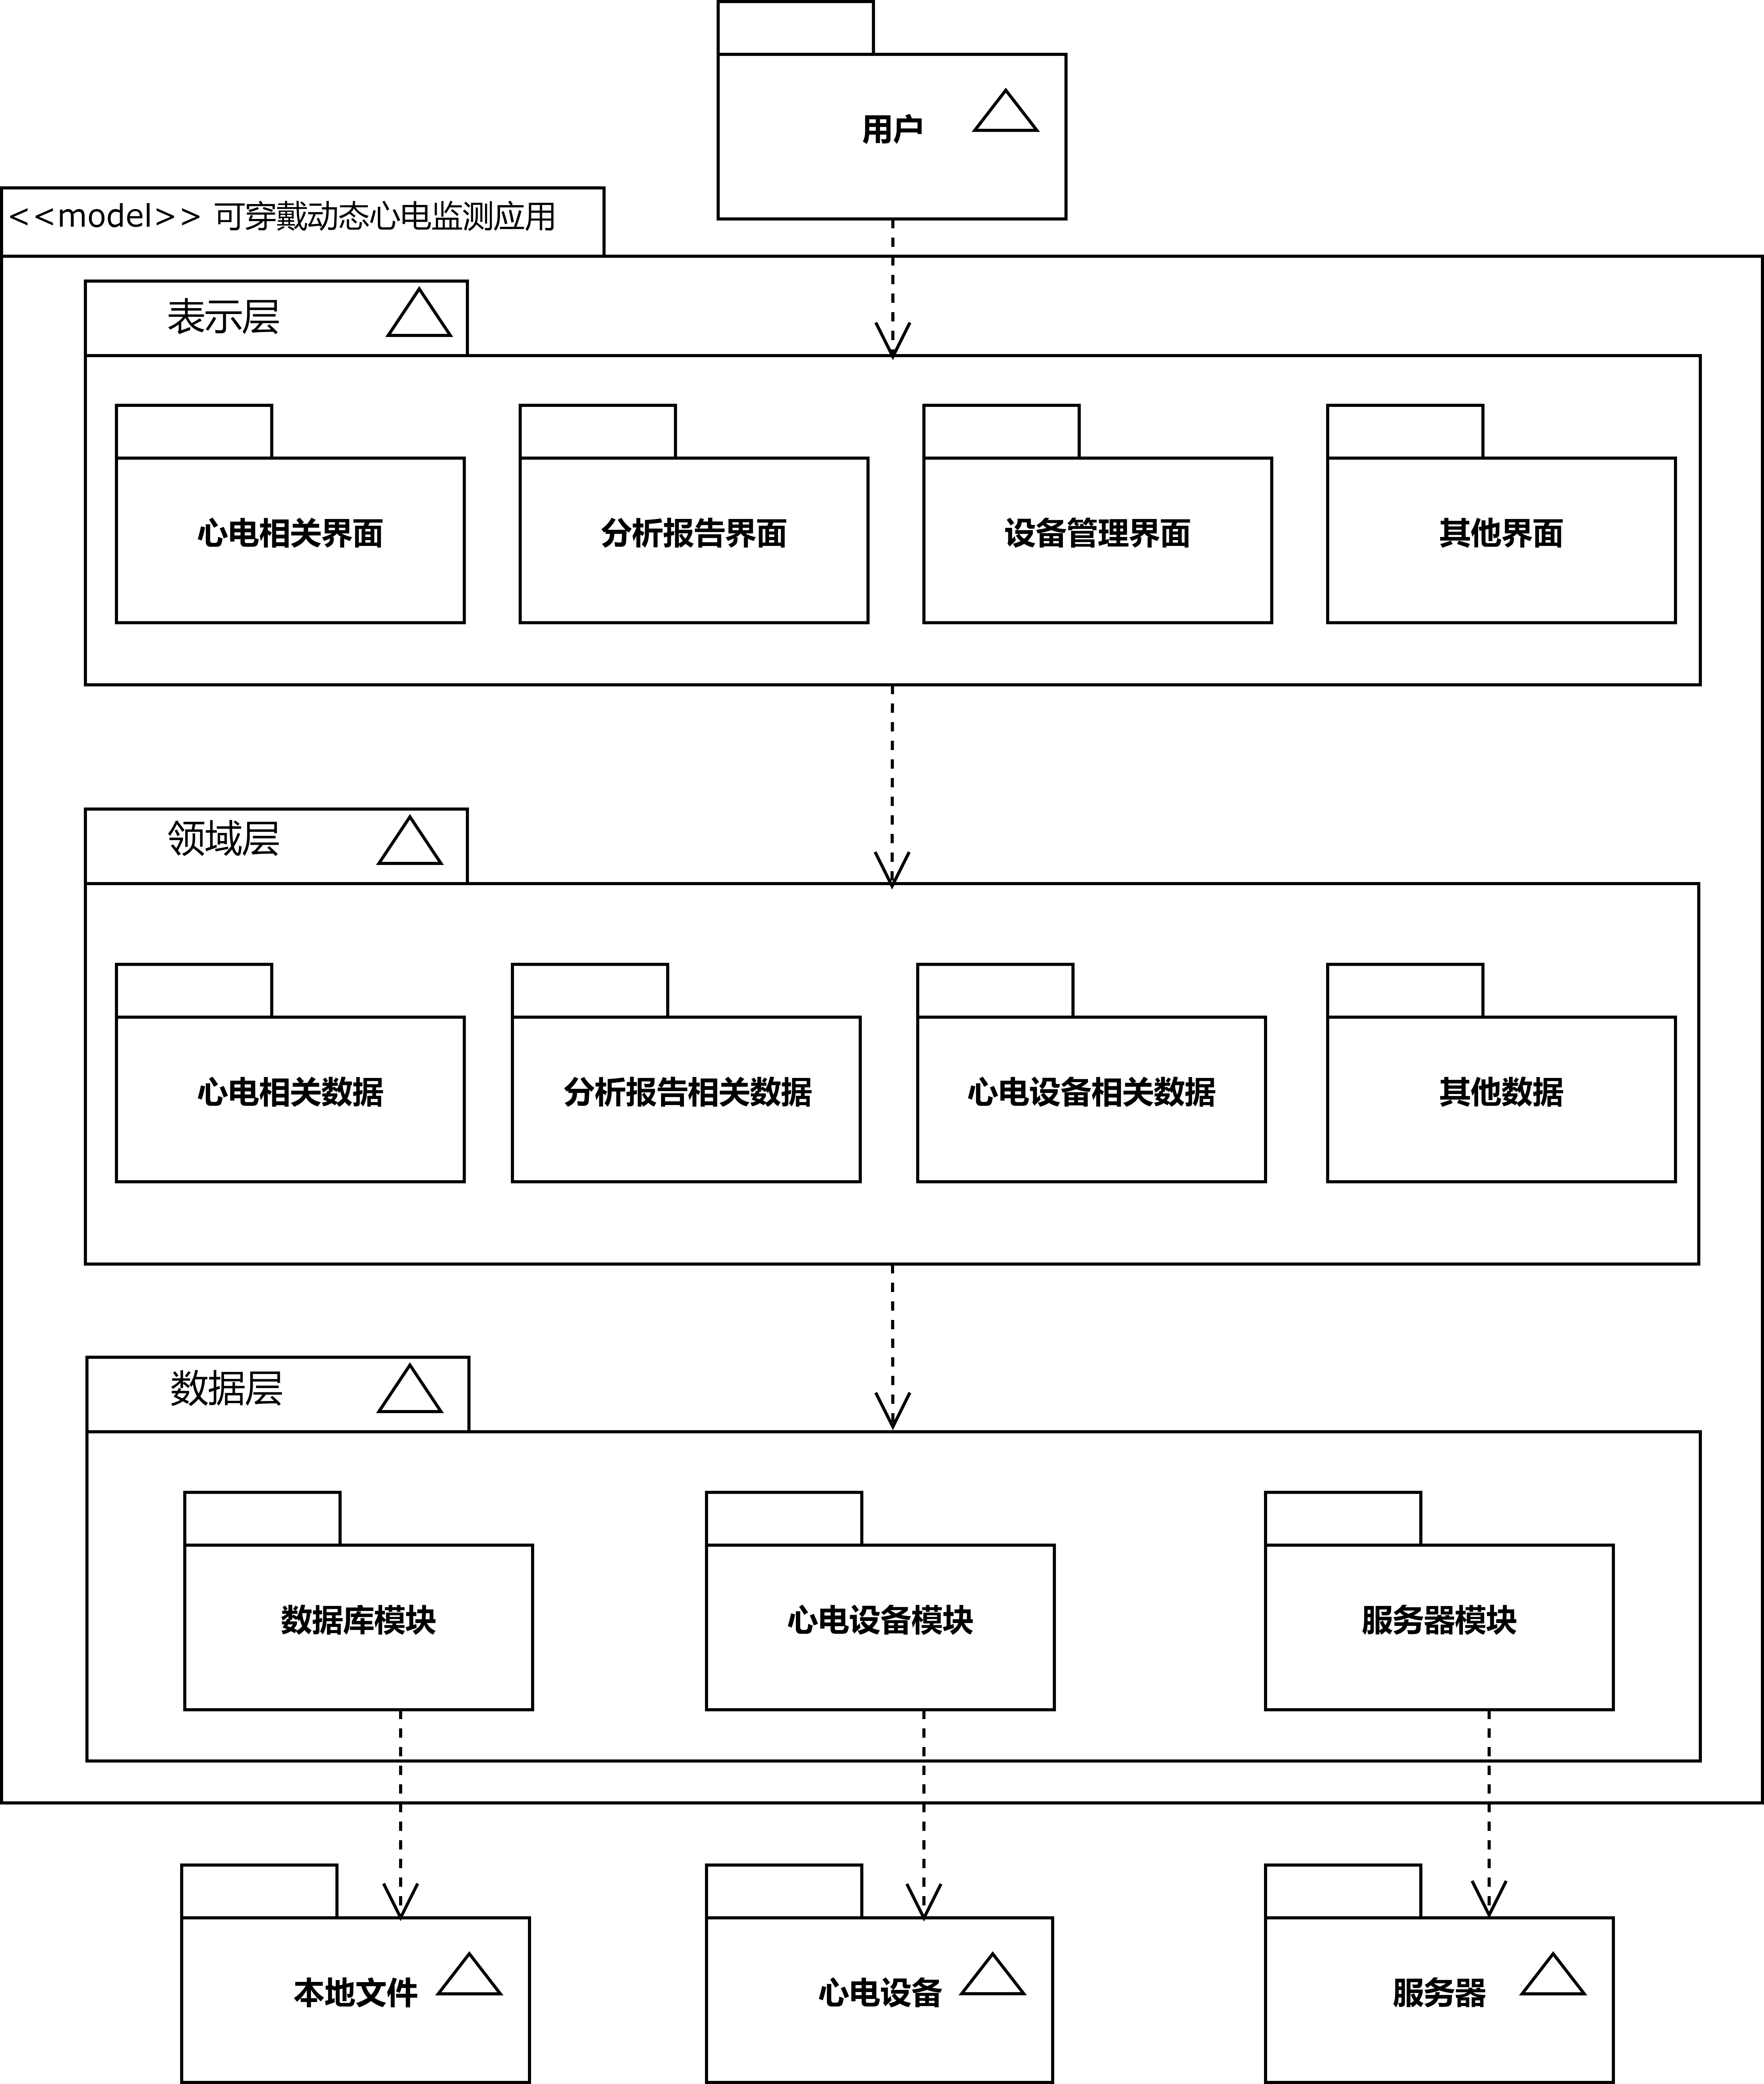
\includegraphics[width=.9\textwidth]{../assets/model.drawio}
    \bicaption{应用的整体架构}{Architecture of the app}
    \label{fig:model}
\end{figure}

本应用使用了Riverpod架构模式\cite{bizzottoFlutterAppArchitecture},其与MVC等传统模式有较大差别,且由于提出较晚而知名度不高,因此本节顺带对该模式进行简单介绍。

在设计应用程序时选择正确的应用架构至关重要,过于简陋的设计会使得代码整体缺乏组织性,过于繁复的设计则会阻碍代码的修改迭代。自最经典的MVC架构以来,已有许多流行的应用架构被相继提出。其中一些对原始的MVC架构进行改动后仍沿用其名称,导致MVC这一术语的含义愈加模糊;另一些变体则被命名为MVP、MVVM、MVC+S等MV*,或是如Clean Architecture等另起炉灶。这些经典的架构模式很难原样照搬至Flutter框架,即使强行在Flutter中进行实现也只会使得代码结构不伦不类。在探索Flutter适用的应用架构的过程中,社区已经提出了许多新模式,如BLoC、Stacked等。而在本应用的架构设计中,采用的则是Andrea于2022年初提出的Riverpod架构模式。

Flutter曾经有一个流行的状态管理包Provider,该包也是上述的BLoC、Stacked等架构模式的基础。后来,由于Provider包的设计逐渐暴露出一些难以解决的问题,其开发者将该包进行了大幅重写,并因其与旧版本不兼容而改名为Riverpod(对Provider中字母的重组)重新发布,Andrea提出的该架构模式因基于Riverpod包而命名为Riverpod架构模式。

该架构由四层组成,从上至下分别是表示(Presentation)层、应用(Application)层、领域(Domain)层、数据(Data)层。

\subsection{表示层}\label{subsec:presentation-layer}

表示层类似于MVC中的View和Controller,或是MVVM中的View和ViewModel,以及Android应用架构指南\footnote{\url{https://developer.android.com/jetpack/guide\#recommended-app-arch}}中的UI层。该层包含用户可见的UI组件以及相关的特定于某个组件的状态与交互逻辑。由于Flutter采用了响应式的设计思想,UI本身与其对应的状态的关系极为密切,因此在Riverpod架构中,将MV*中的Model以外的两层进行了合并。在本应用中,该层包含实时心电界面、历史心电界面、分析报告界面等内容。

\subsection{应用层}\label{subsec:app-layer}

应用层类似Android应用架构指南中的领域层(两边对领域层这一术语的使用不一致),并且与其一样是可选的。这是因为并非所有应用都具有复杂的业务逻辑,也并非所有业务逻辑都需要被提取出来以便重用。在Riverpod架构中,如果不需要应用层,则可以直接省略这一层。在本应用中,由于应用的业务逻辑较为简单,因此并未使用该层。

\subsection{领域层}\label{subsec:domain-layer}

领域层类似于MV*中的Model。该层包含领域模型,即应用程序中的数据及其相关的方法。由于领域层在各种架构模式中被广泛使用(尽管命名可能不同),此处不作详细介绍。在本应用中,该层包括心电数据、心拍数据、应用设置数据等模型。

\subsection{数据层}\label{subsec:data-layer}

数据层类似Android应用架构指南中的数据层。该层包含与外部数据源通信的相关代码,负责将领域模型与底层的数据源的实现细节进行隔离,将从数据源获取的原始格式的数据(如JSON等)转换为领域层中的领域对象(应用中自定义的数据类),有时也执行数据缓存等操作。在本应用中,该层包含与数据库、心电监测设备、服务器进行通信的相关代码。


\section{应用各个模块的设计}\label{sec:app-design}

\subsection{心电模块的设计}\label{subsec:ecg-design}

\todo{心电模块的设计}

\subsection{分析报告界面的设计}\label{subsec:analytics-design}

分析报告界面的整体外观如图~\ref{fig:analytics} 所示。在导航栏中为分析报告使用了表示数据分析的图标。

\begin{figure}[ht]
    \subcaptionbox{加载中}{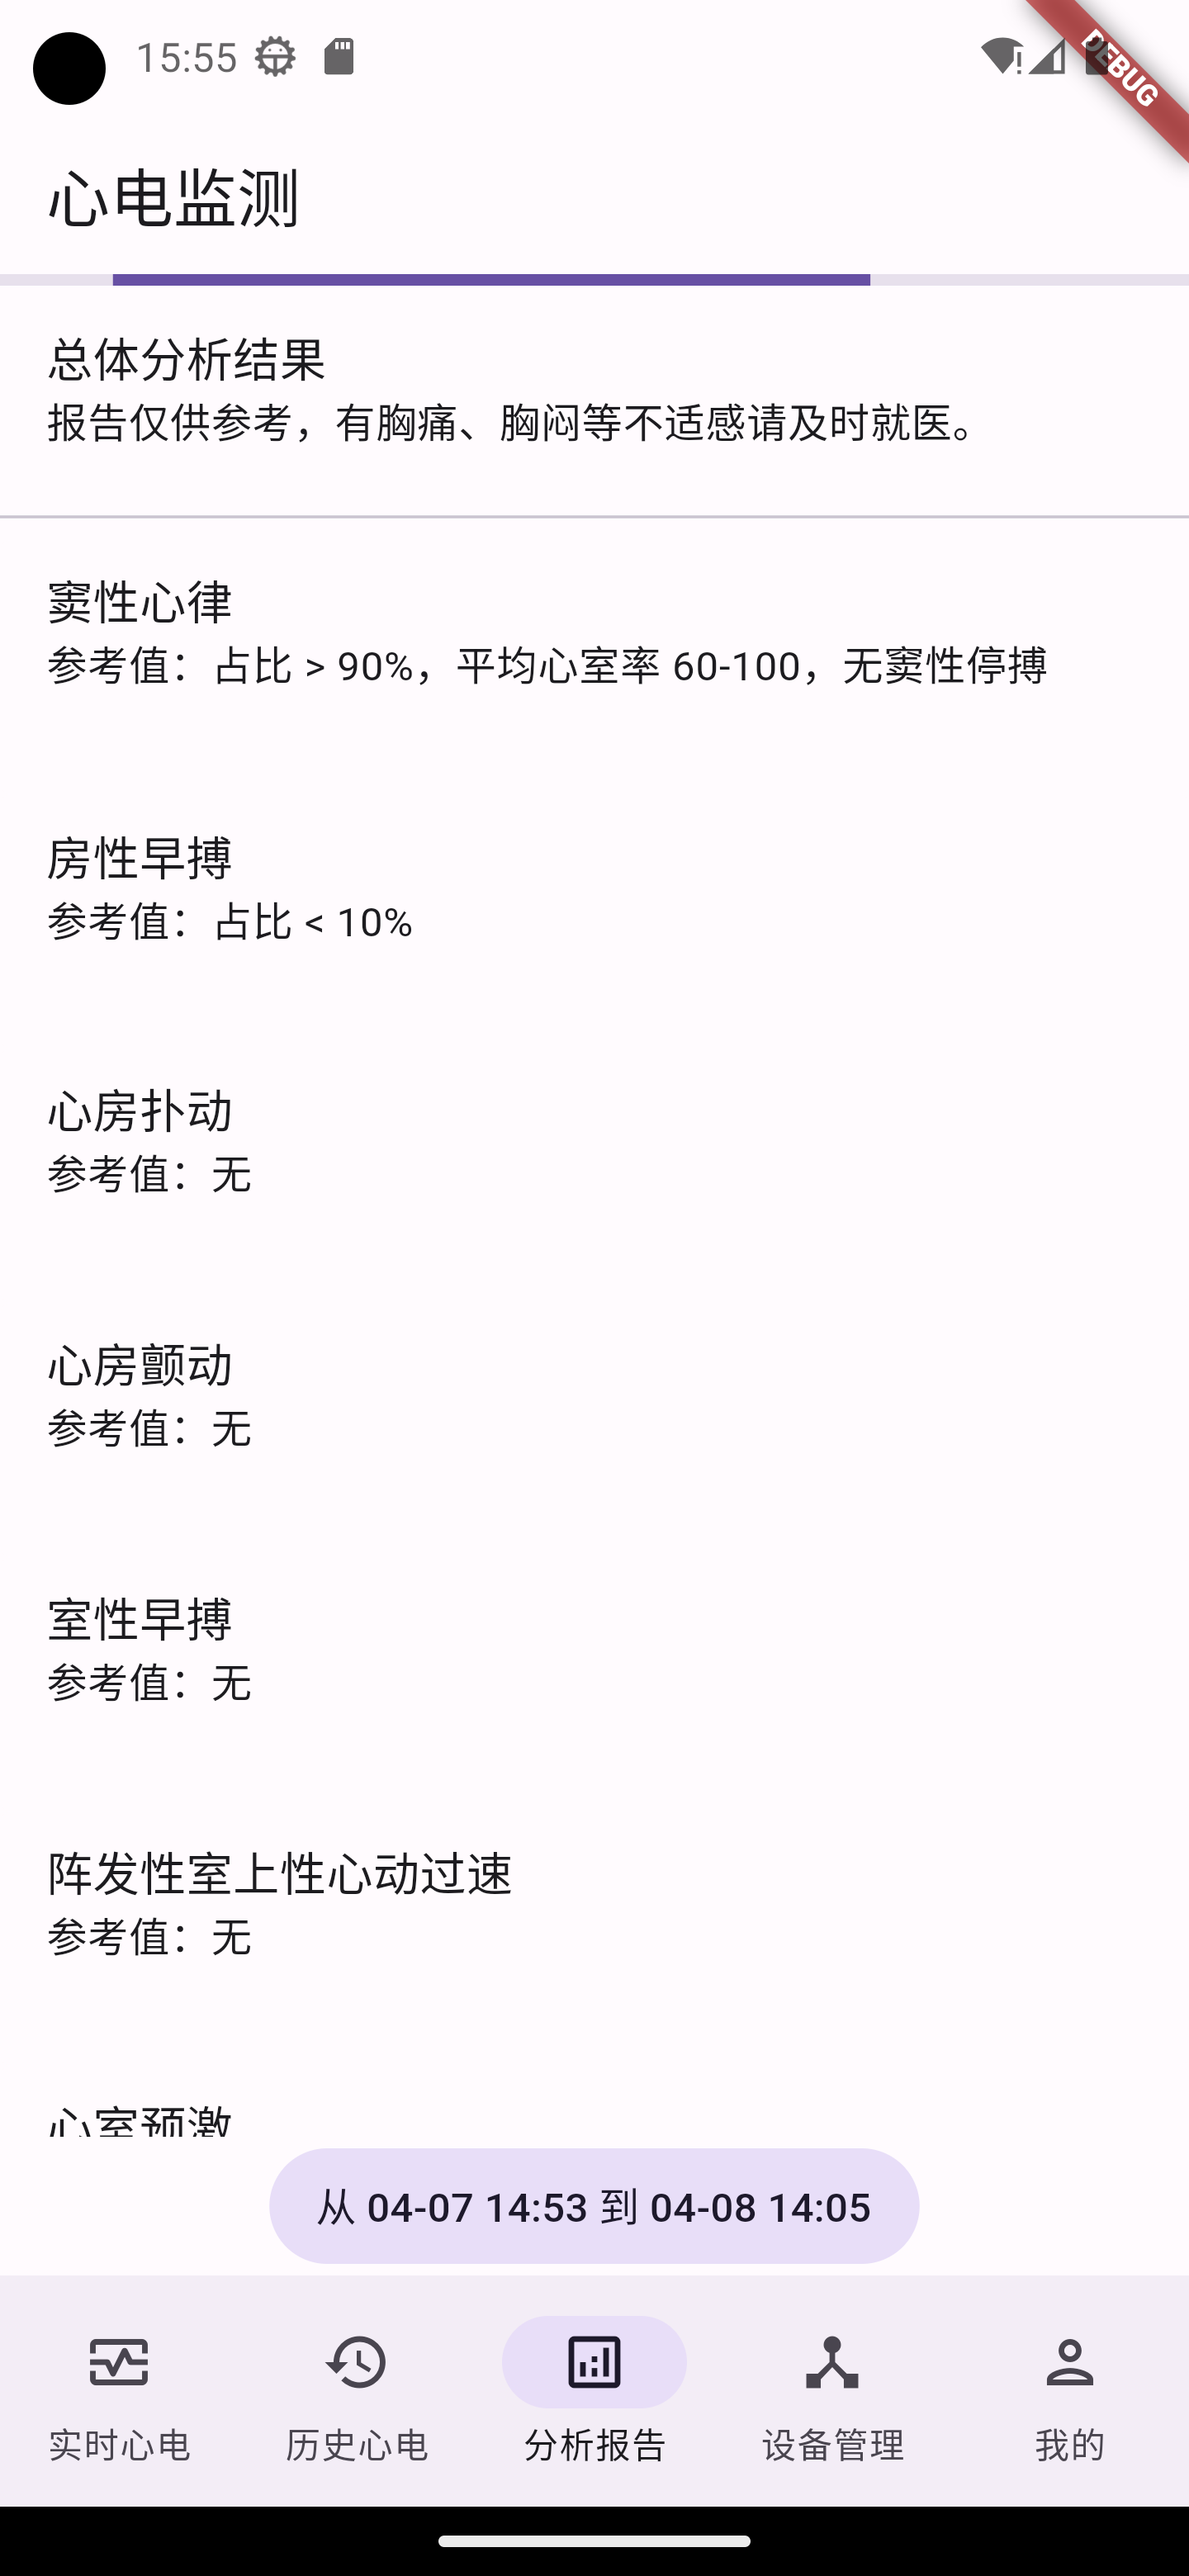
\includegraphics[width=.33\textwidth]{../assets/analytics-loading}}
    \subcaptionbox{正常状态}{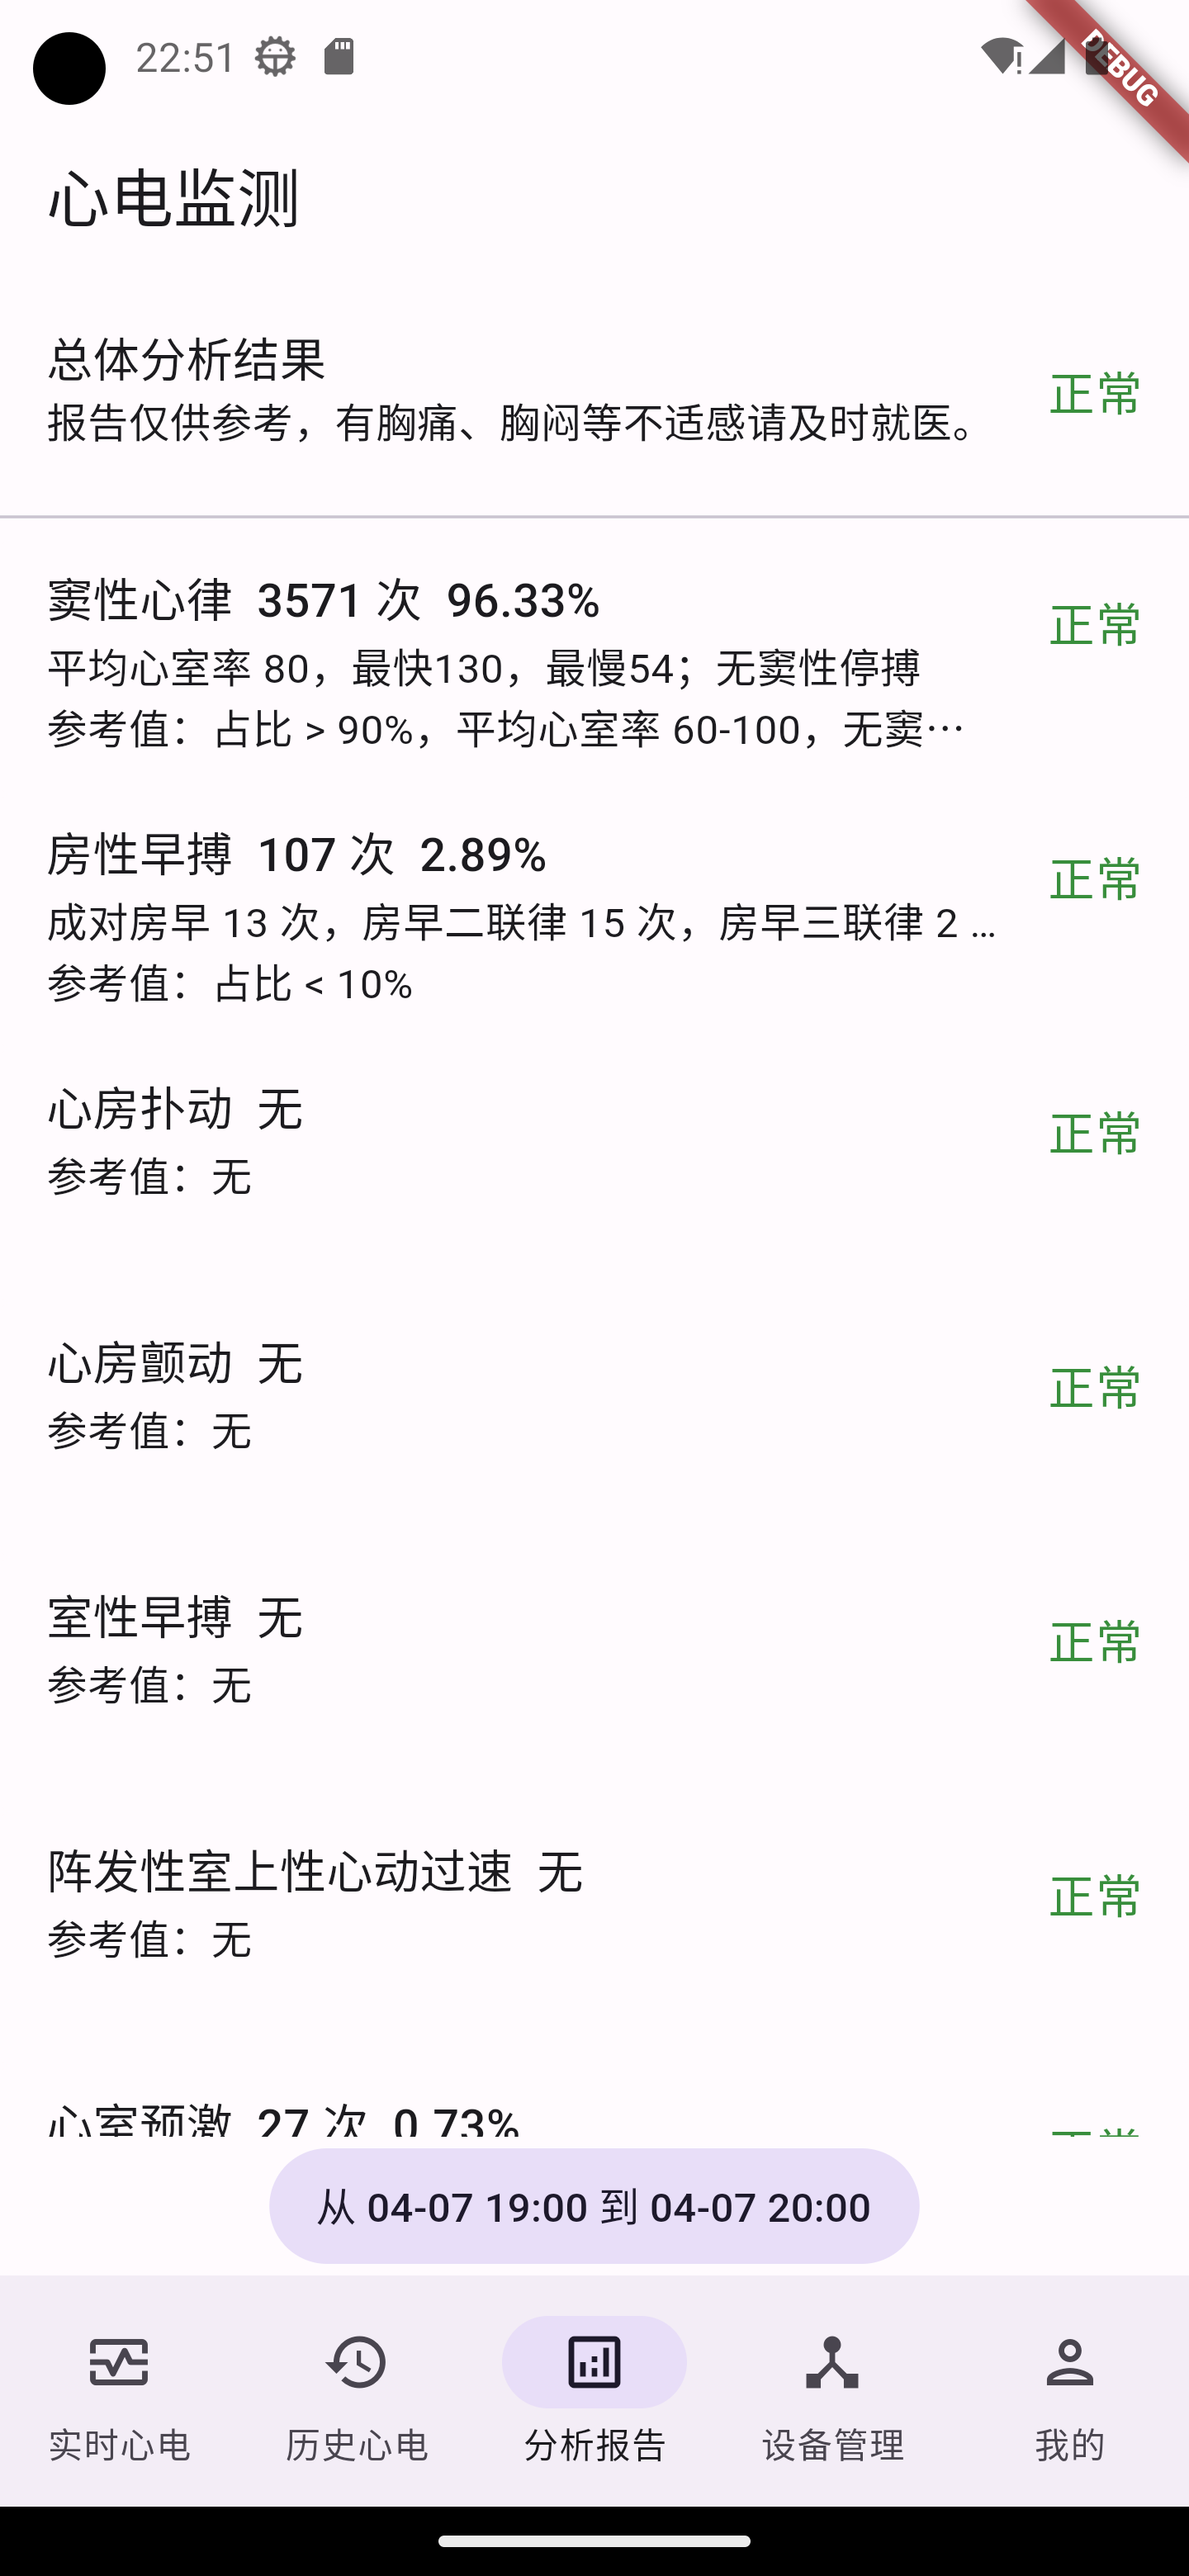
\includegraphics[width=.33\textwidth]{../assets/analytics}}
    \subcaptionbox{时间范围选择}{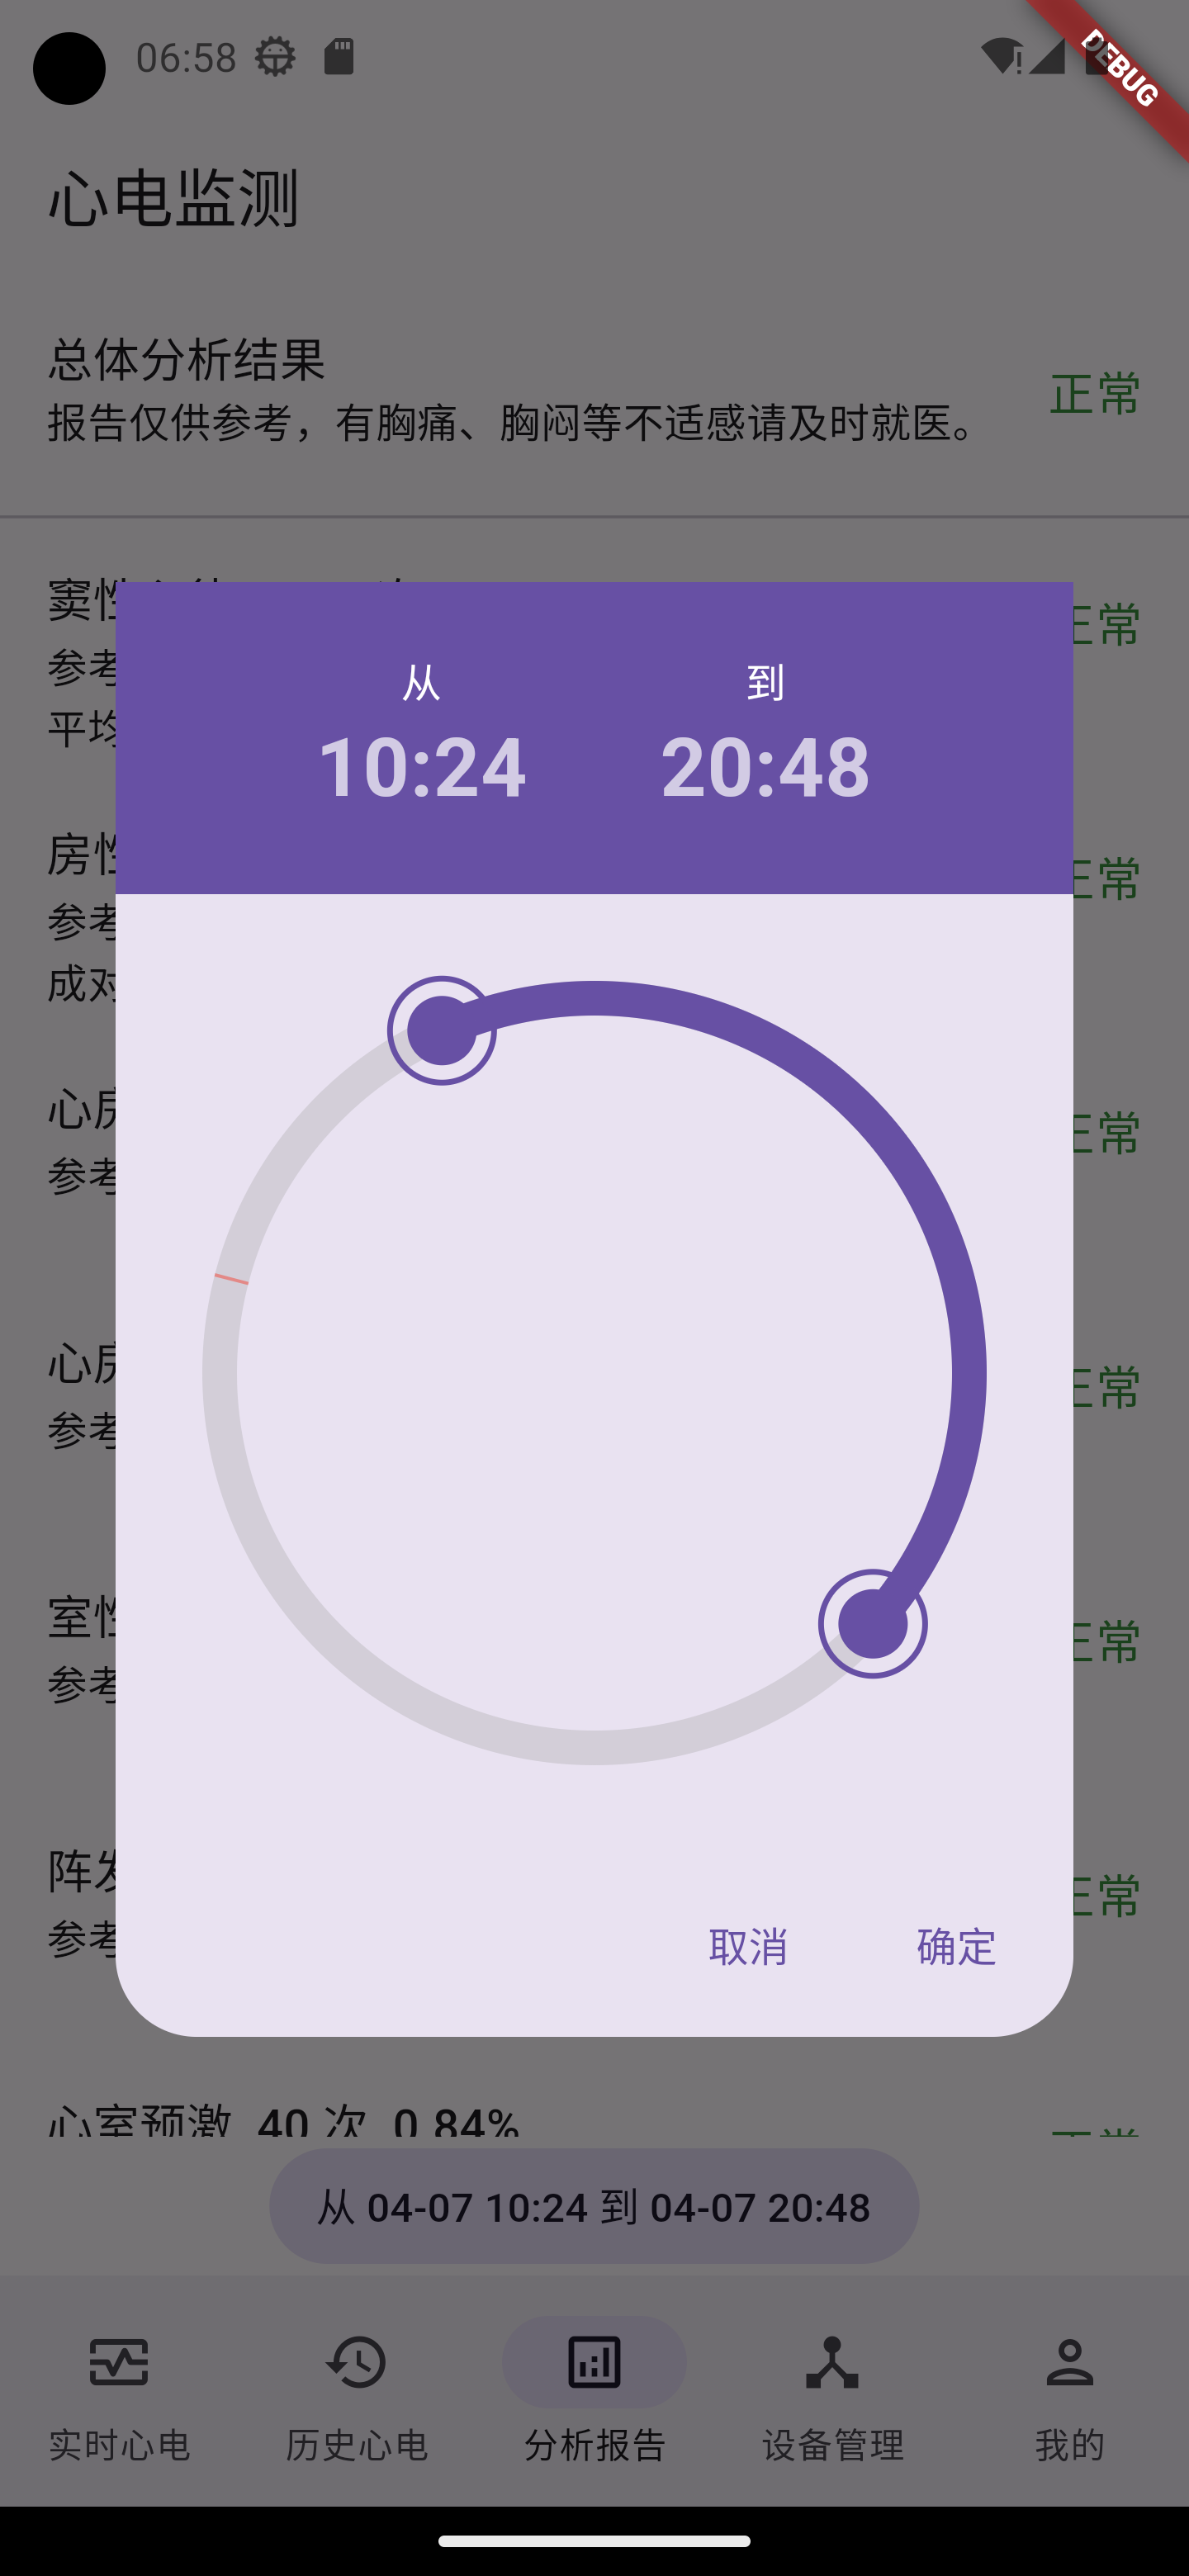
\includegraphics[width=.33\textwidth]{../assets/analytics-dialog}}
    \bicaption{分析报告界面的截图}{Screenshot of the analytics page}
    \label{fig:analytics}
\end{figure}

该界面可以划分为分析报告展示与时间范围选择器两部分,另外点击心律类型可以展开心律类型详情界面。

\subsubsection{分析报告展示部分的设计}\label{subsubsec:analytics-display-design}

该部分区域整体上是一个可以上下滑动的列表。由于分析报告内容过多,在一个屏幕内完全展示会过于拥挤,所以使用了可滑动列表的形式。

最上方的一小条区域是线状进度指示器。由于难以确定生成分析报告所需的具体时长,所以该进度指示器是不确定进度的样式。另外,由于该部分有很多界面元素可以在获取到实际数据之前就确认其内容与位置,所以没有像历史心电界面那样使用屏幕中央的圆形加载进度指示器,而只是在最上方使用了线状进度指示器,并在加载时提前显示部分可以确定的元素,以减少加载前后的界面变化,提升用户对界面内容的确定感。在加载完成后,该区域并不会直接消失,而是会替换为不可见的与进度指示器高度相同的空白元素,以保证界面布局的稳定性,避免下方内容在加载完成后突然上移。

在进度指示器之下显示了所选时间范围的分析结果的总结,以右侧以带颜色的字体显示对分析结果的简要概括(“正常”、“心动过速”等),并在下方给出稍详细一些的解释。

总结区域的下方放置了一条分割线,用以分割总体分析结果与具体的心律类型分析结果,并在视觉上对总体结果加以适当强调。

在分割线之下,每个心律类型的分析结果都会显示在一个独立的区域中。首先以稍大的字体显示心律类型的名称、次数、占比,然后以小一些的字体给出该心律类型相关数据的正常范围作为参考值,第三行显示部分心律类型会具有的额外信息,如成对房早次数等;后两行的内容各自被限制在一行之内,溢出的内容会被以省略号替代,以提示用户可以点击该区域查看更多信息。此外,每个心律类型的右侧也和总结一样给出了对该心律类型分析结果的简要概括。

各个心律类型的区域都是可以点击展开查看详细信息的。通常而言,可点击区域应当使用按钮等样式加以指示,但当屏幕上的可点击区域过多时应该避免过多的装饰,以免造成视觉上的混乱。对于列表项的可点击性的指示,一种常见的做法是在右侧显示一个箭头,但在本界面中右侧已经被占据,不便添加更多元素。因此,本界面使用了其他方式来提醒用户心律类型可以点击。除上文所述的省略号外,该界面利用下方被截断的列表项指示该区域可以滑动查看更多内容,并在用户滑过心律区域时展示了水墨扩散的效果,如图~\ref{fig:ink} 所示,效果会从点击位置向四周扩散。水墨扩散效果在Material设计中用于各种可点击区域的反馈,可以提醒用户心律展示区域点击后能触发额外动作。

\begin{figure}[ht]
    \centering
    
\includegraphics[width=.5\textwidth]{../assets/ink}
    \bicaption{心律类型区域的水墨扩散效果}{Ink effect of the heart rhythm area}
    \label{fig:ink}
\end{figure}

\subsubsection{时间范围选择器部分的设计}\label{subsubsec:analytics-time-range-design}

时间范围选择器部分仅在中间包含一个填充色调按钮。因为需要明确提醒用户所示分析报告的时间范围,所以没有使用强调效果较弱的轮廓按钮和文本按钮。按钮中的文本指示了当前选择的时间范围。点击按钮后,会弹出时间范围选择对话框。

时间范围选择对话框的主体是一个圆环,用户可以拖动圆环上的两个点来选定分析范围的起止时间。为了不引起日期的混淆,当前时间(在圆环上显示为红色)不被允许包含在选择部分之中,这样可以保证用户所选的时间范围总是可以解释为过去24小时之内的某个时间段。

\subsubsection{心律类型详情界面的设计}\label{subsubsec:label-details}

心律类型详情界面的整体外观的如图~\ref{fig:label-details} 所示。除上方的心律名称和返回按钮外,界面由可滑动查看的列表构成。列表内容包括该心律类型的说明文本,以及心律出现的具体时间。为了保证每个时间都可以较容易点击到,时间之间留有适当的间隔。点击时间后,会跳转至历史心电的对应时间。

\begin{figure}[ht]
    \centering
    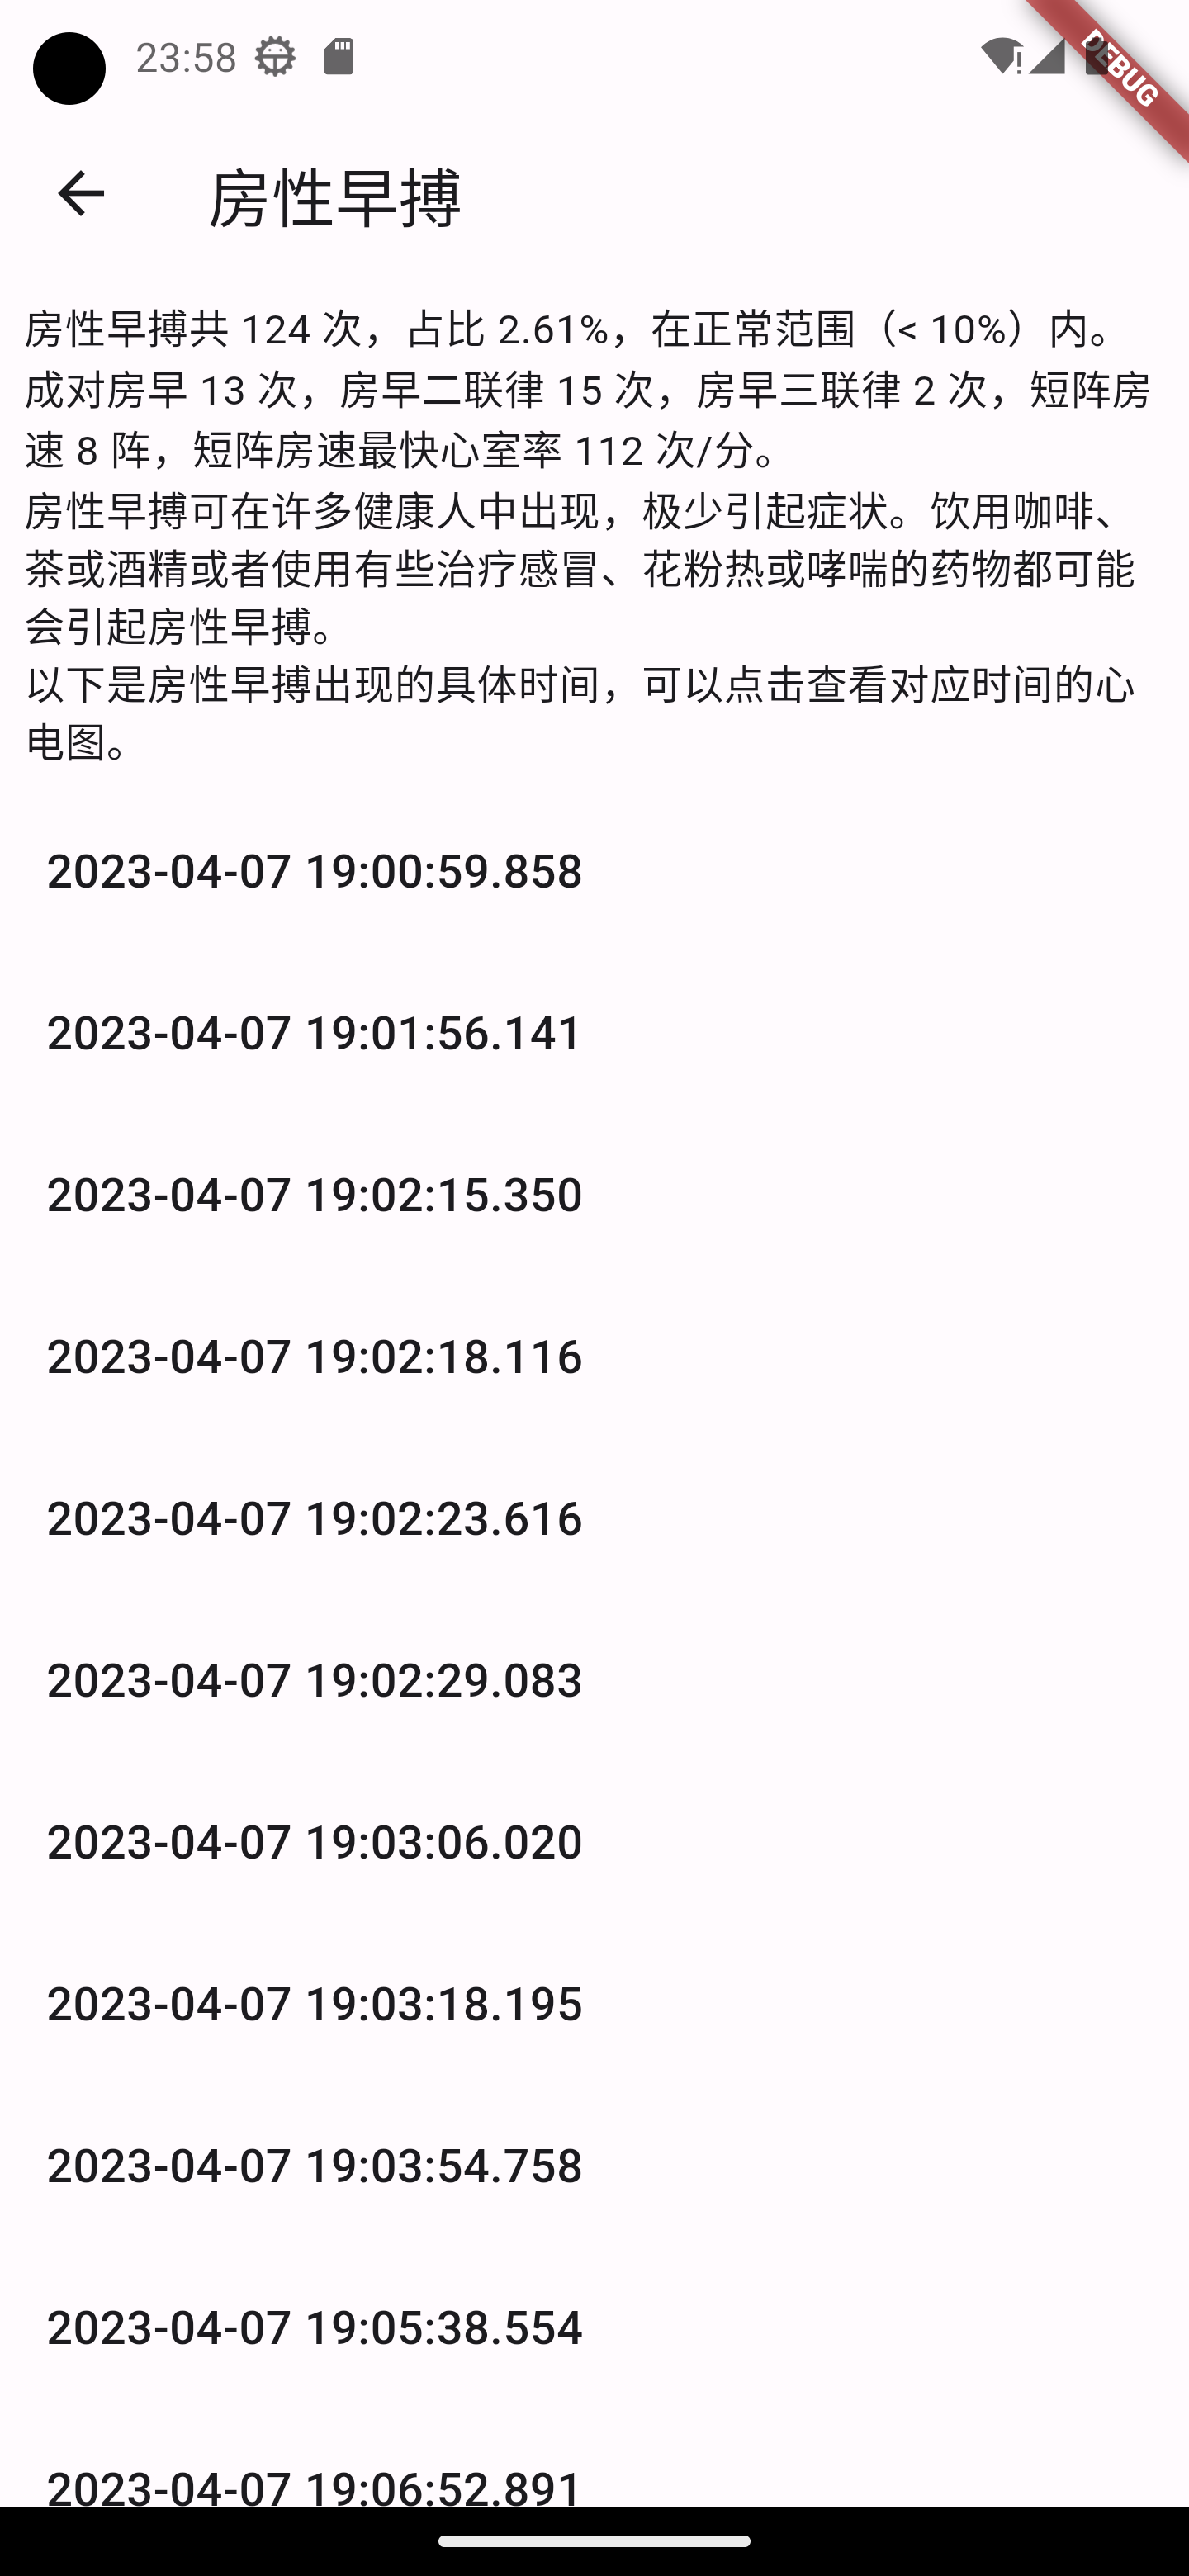
\includegraphics[width=.33\textwidth]{../assets/label-details}
    \bicaption{心律类型详情界面的截图}{Screenshot of the heart rhythm details page}
    \label{fig:label-details}
\end{figure}

\subsection{设备管理界面的设计}\label{subsec:device-design}

\begin{figure}[ht]
    \subcaptionbox{已连接}{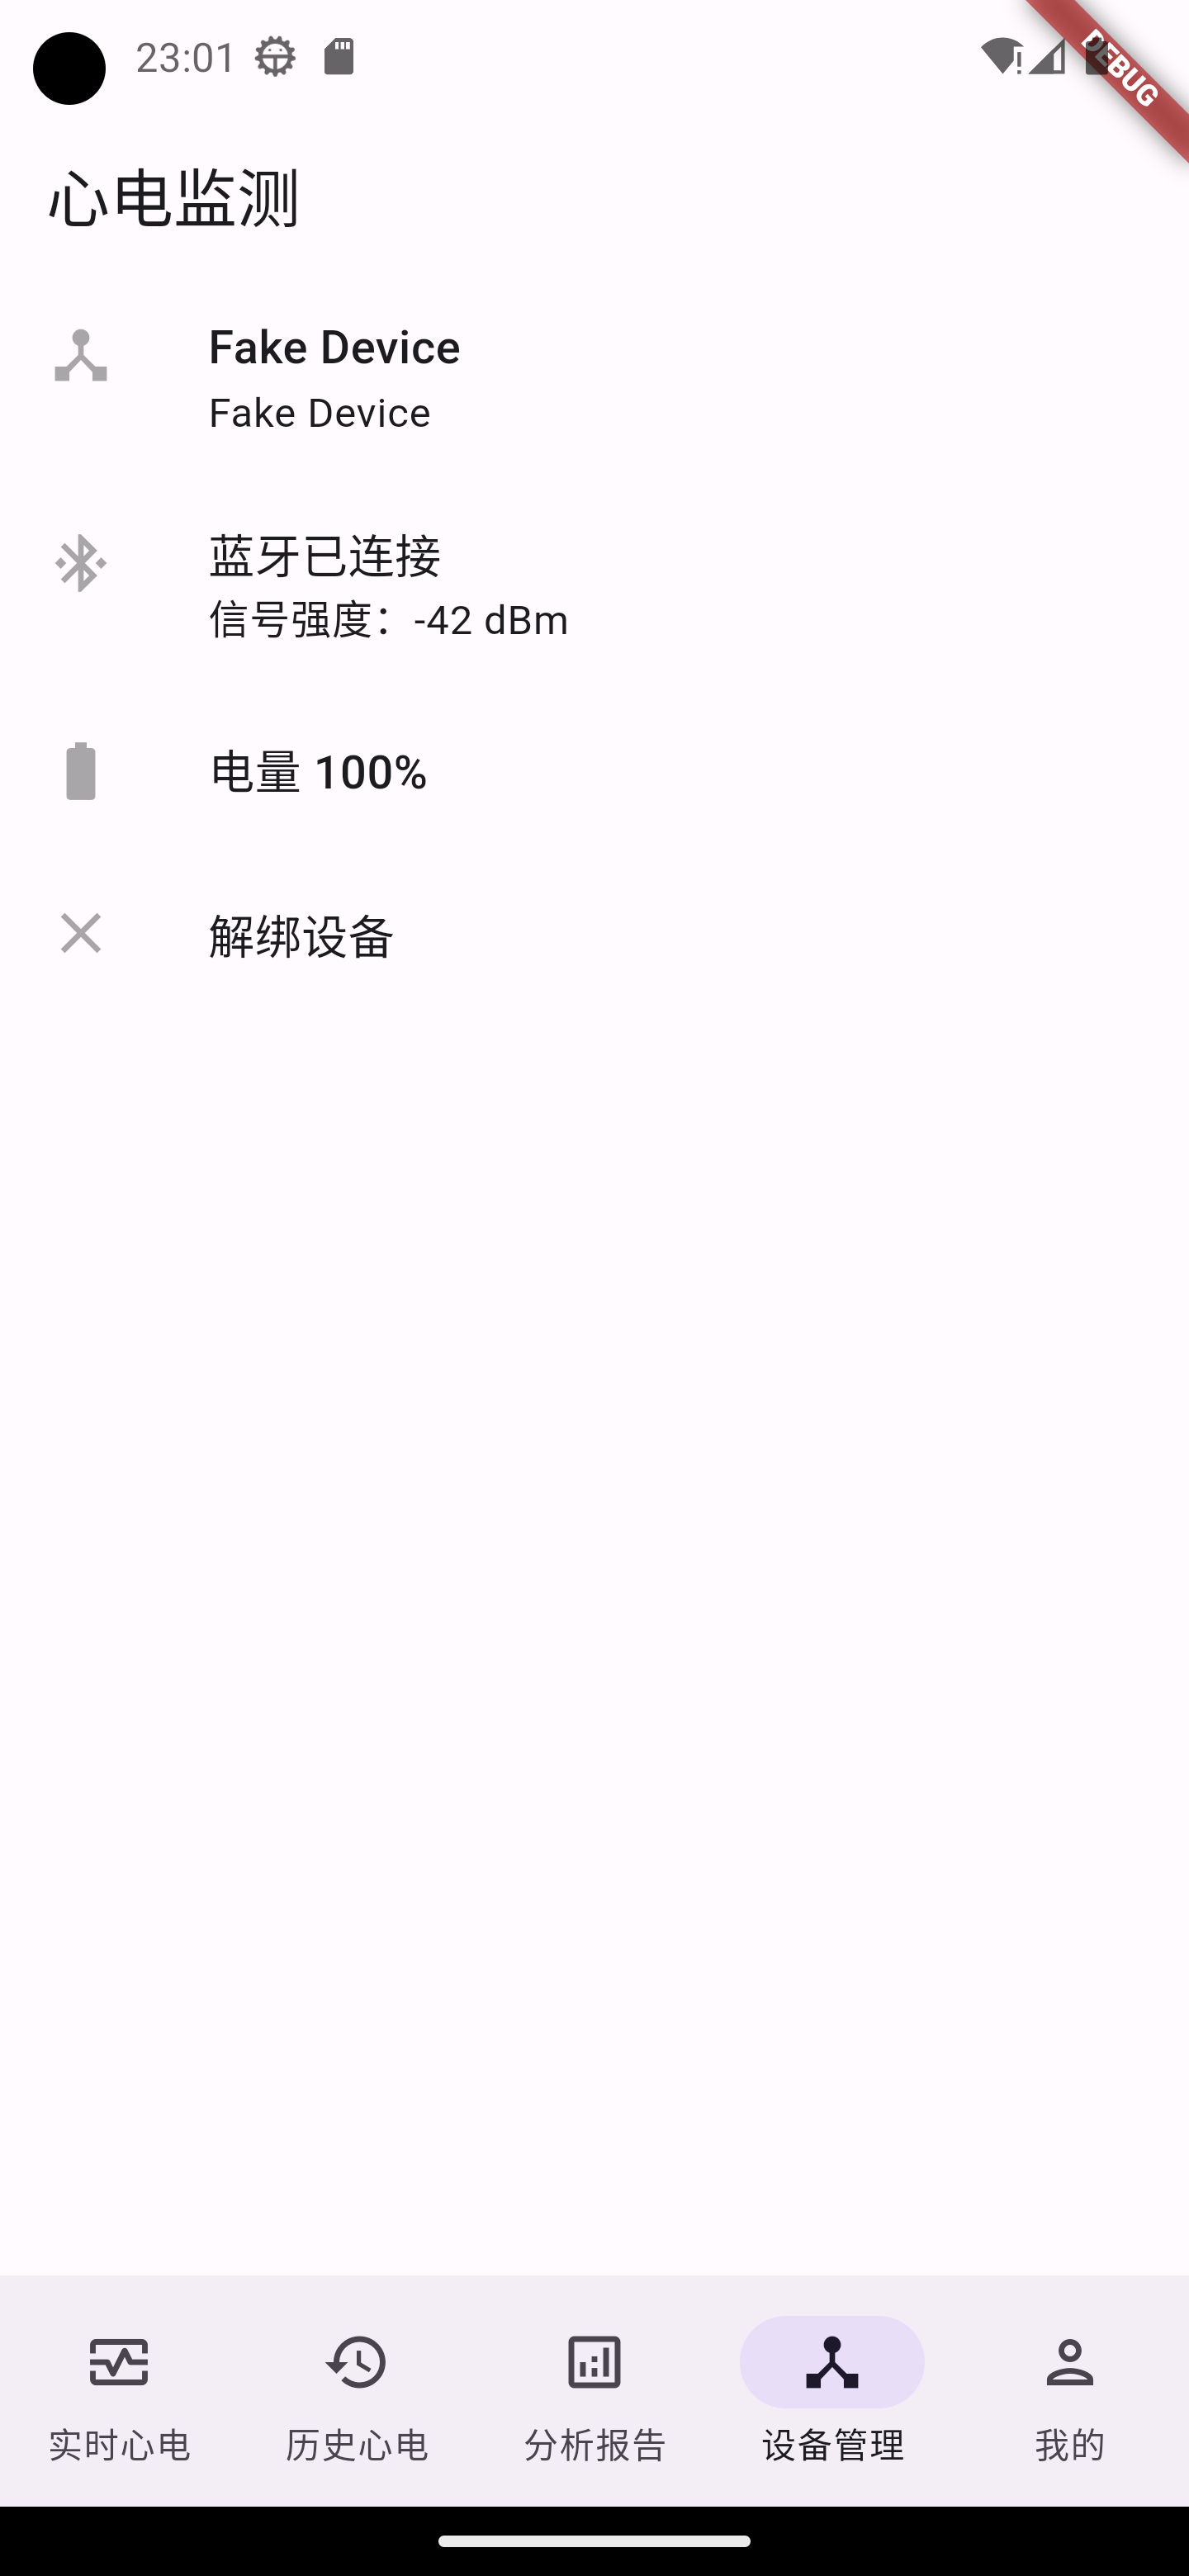
\includegraphics[width=.33\textwidth]{../assets/device-connected}}
    \subcaptionbox{连接新设备}{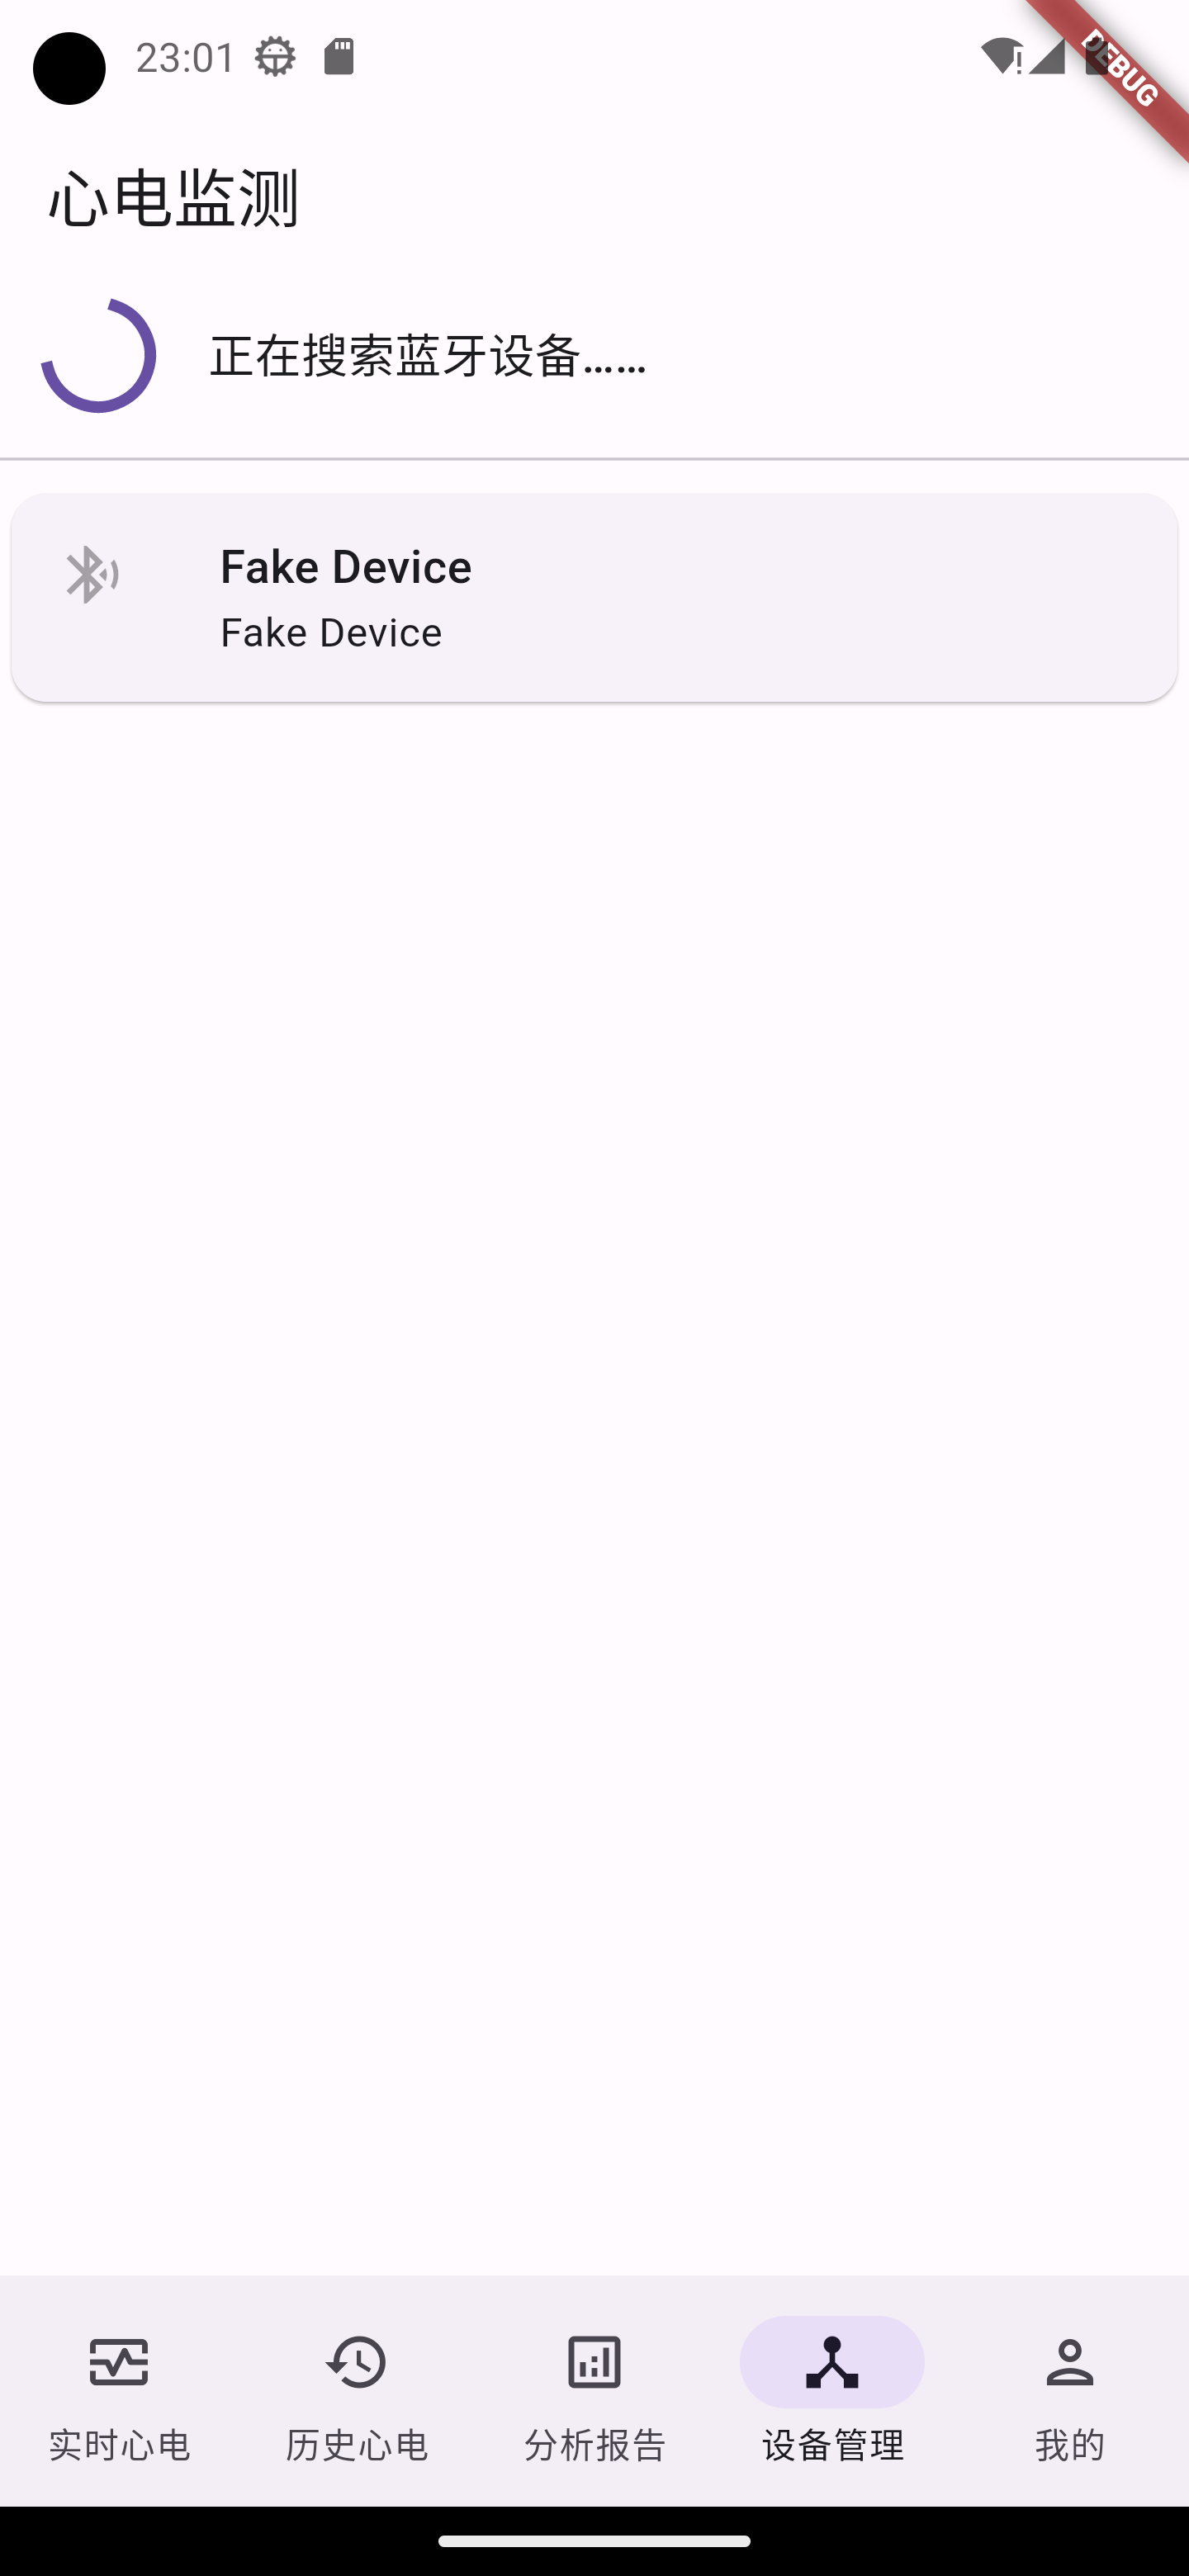
\includegraphics[width=.33\textwidth]{../assets/device-new}}
    \subcaptionbox{无可用设备}{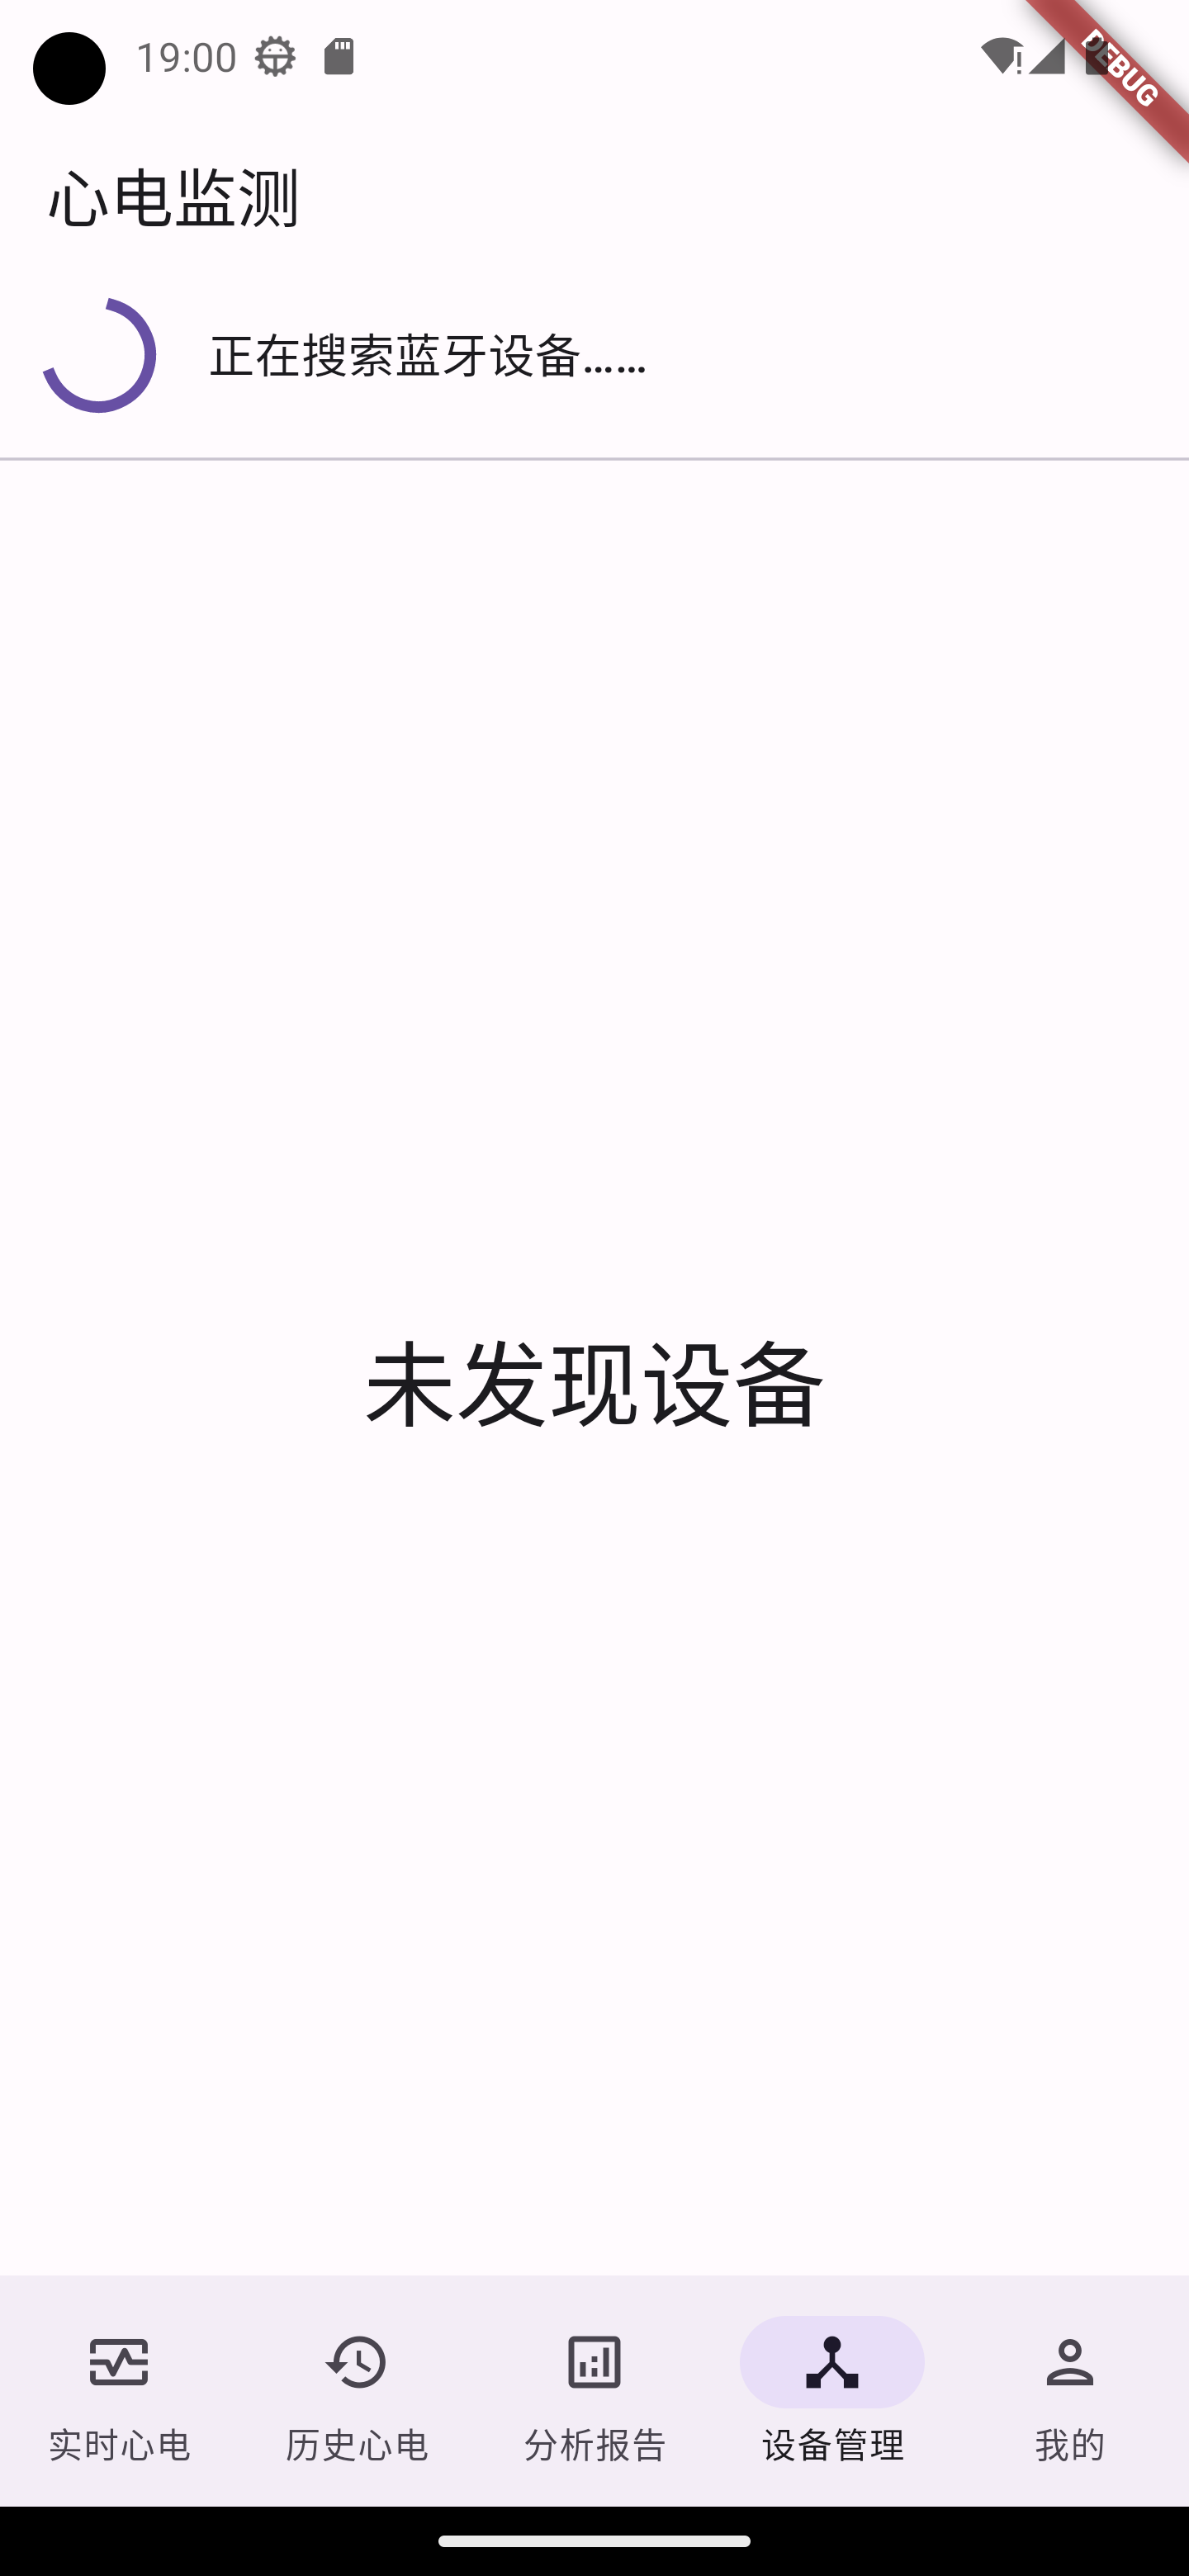
\includegraphics[width=.33\textwidth]{../assets/device-na}}
    \bicaption{设备管理界面的截图}{Screenshot of the device page}
    \label{fig:device}
\end{figure}

设备管理界面的整体外观如图~\ref{fig:device} 所示。设备管理在导航栏中的图标是对心电监测设备所使用的电极片的简化表示。

该界面相比上述其他界面较为简单,分为已绑定设备和未绑定设备两种状态。

在已绑定设备的状态下,该界面会以列表形式展示设备的名称、型号、信号强度、剩余电量与充电状态等信息,并提供解绑设备的按钮。该按钮没有使用额外的设计来表示其可以点击,因为“解绑设备”这一文本本身已经足够明确地指示了该区域是可以点击的。

在未绑定设备的状态下,该界面会起到搜索并绑定设备的作用。界面上方展示“正在搜索蓝牙设备”的提示并显示了不确定进度的圆形进度指示器,之后有一条分割线,下方则展示了搜索到的设备列表。列表中的每一项都表示了一个搜索到的蓝牙设备(由于Android和iOS模拟器均不支持蓝牙功能,截图中仅显示了一个模拟设备),并以带阴影的卡片的样式来显示其可以直接点击,而没有额外放置绑定按钮,以使界面设计更加简洁。

\subsection{其他功能的设计}\label{subsec:other-design}

应用中有一些用户不常主动访问,但仍然应该提供的界面,一些相关界面的外观如图~\ref{fig:other} 所示。

\begin{figure}[ht]
    \subcaptionbox{我的}{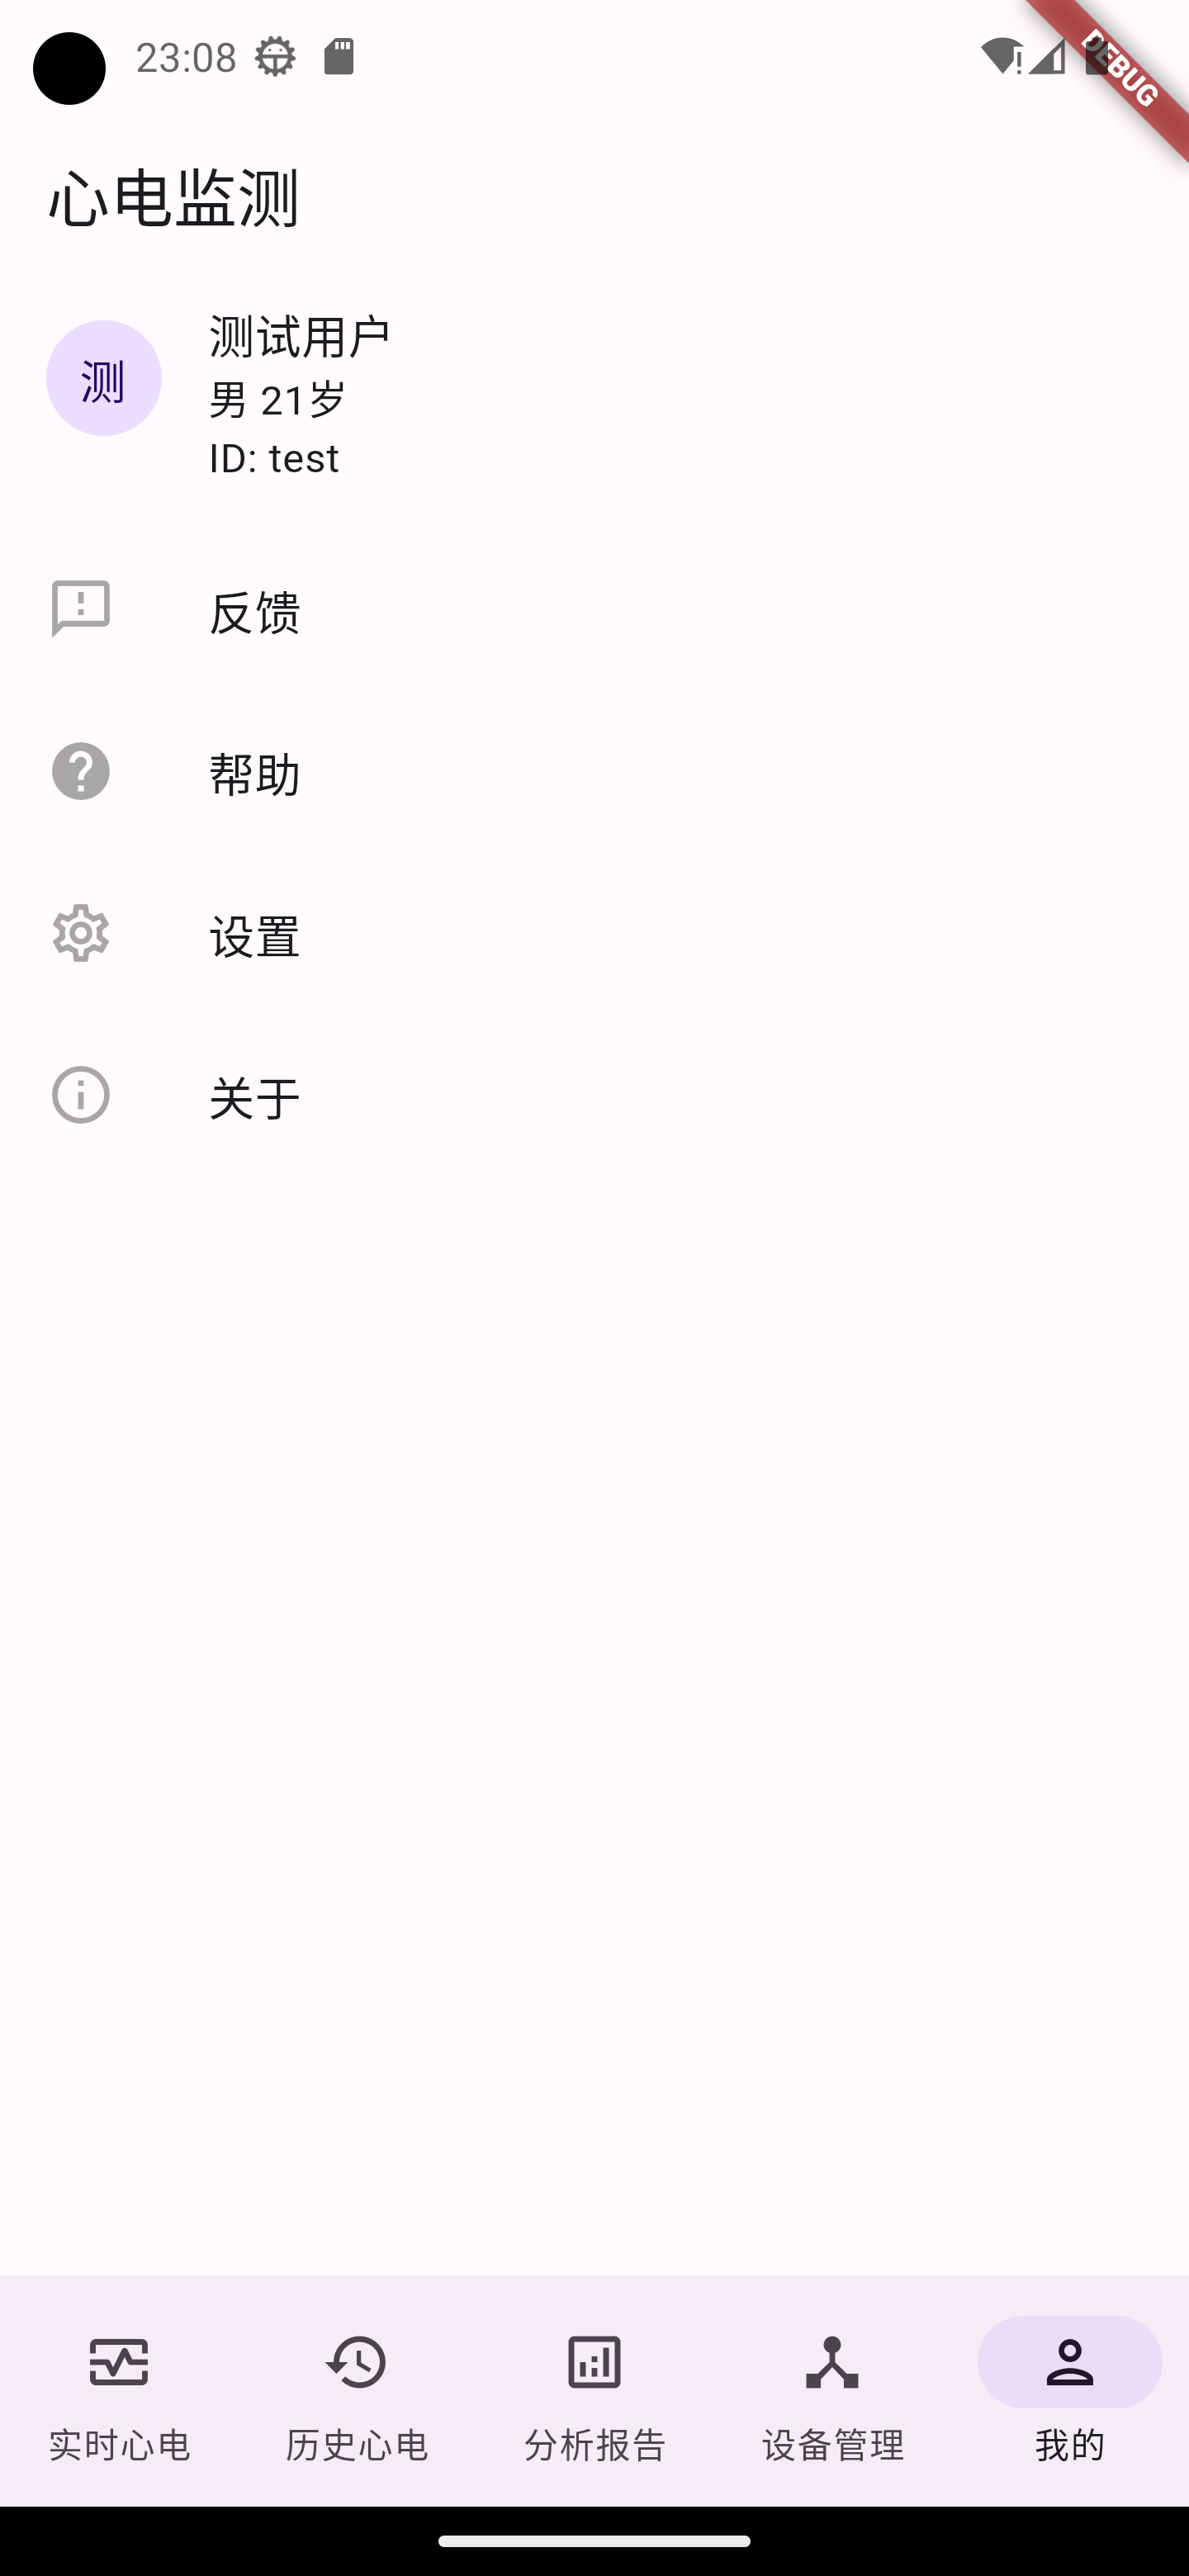
\includegraphics[width=.33\textwidth]{../assets/me}}
    \subcaptionbox{设置}{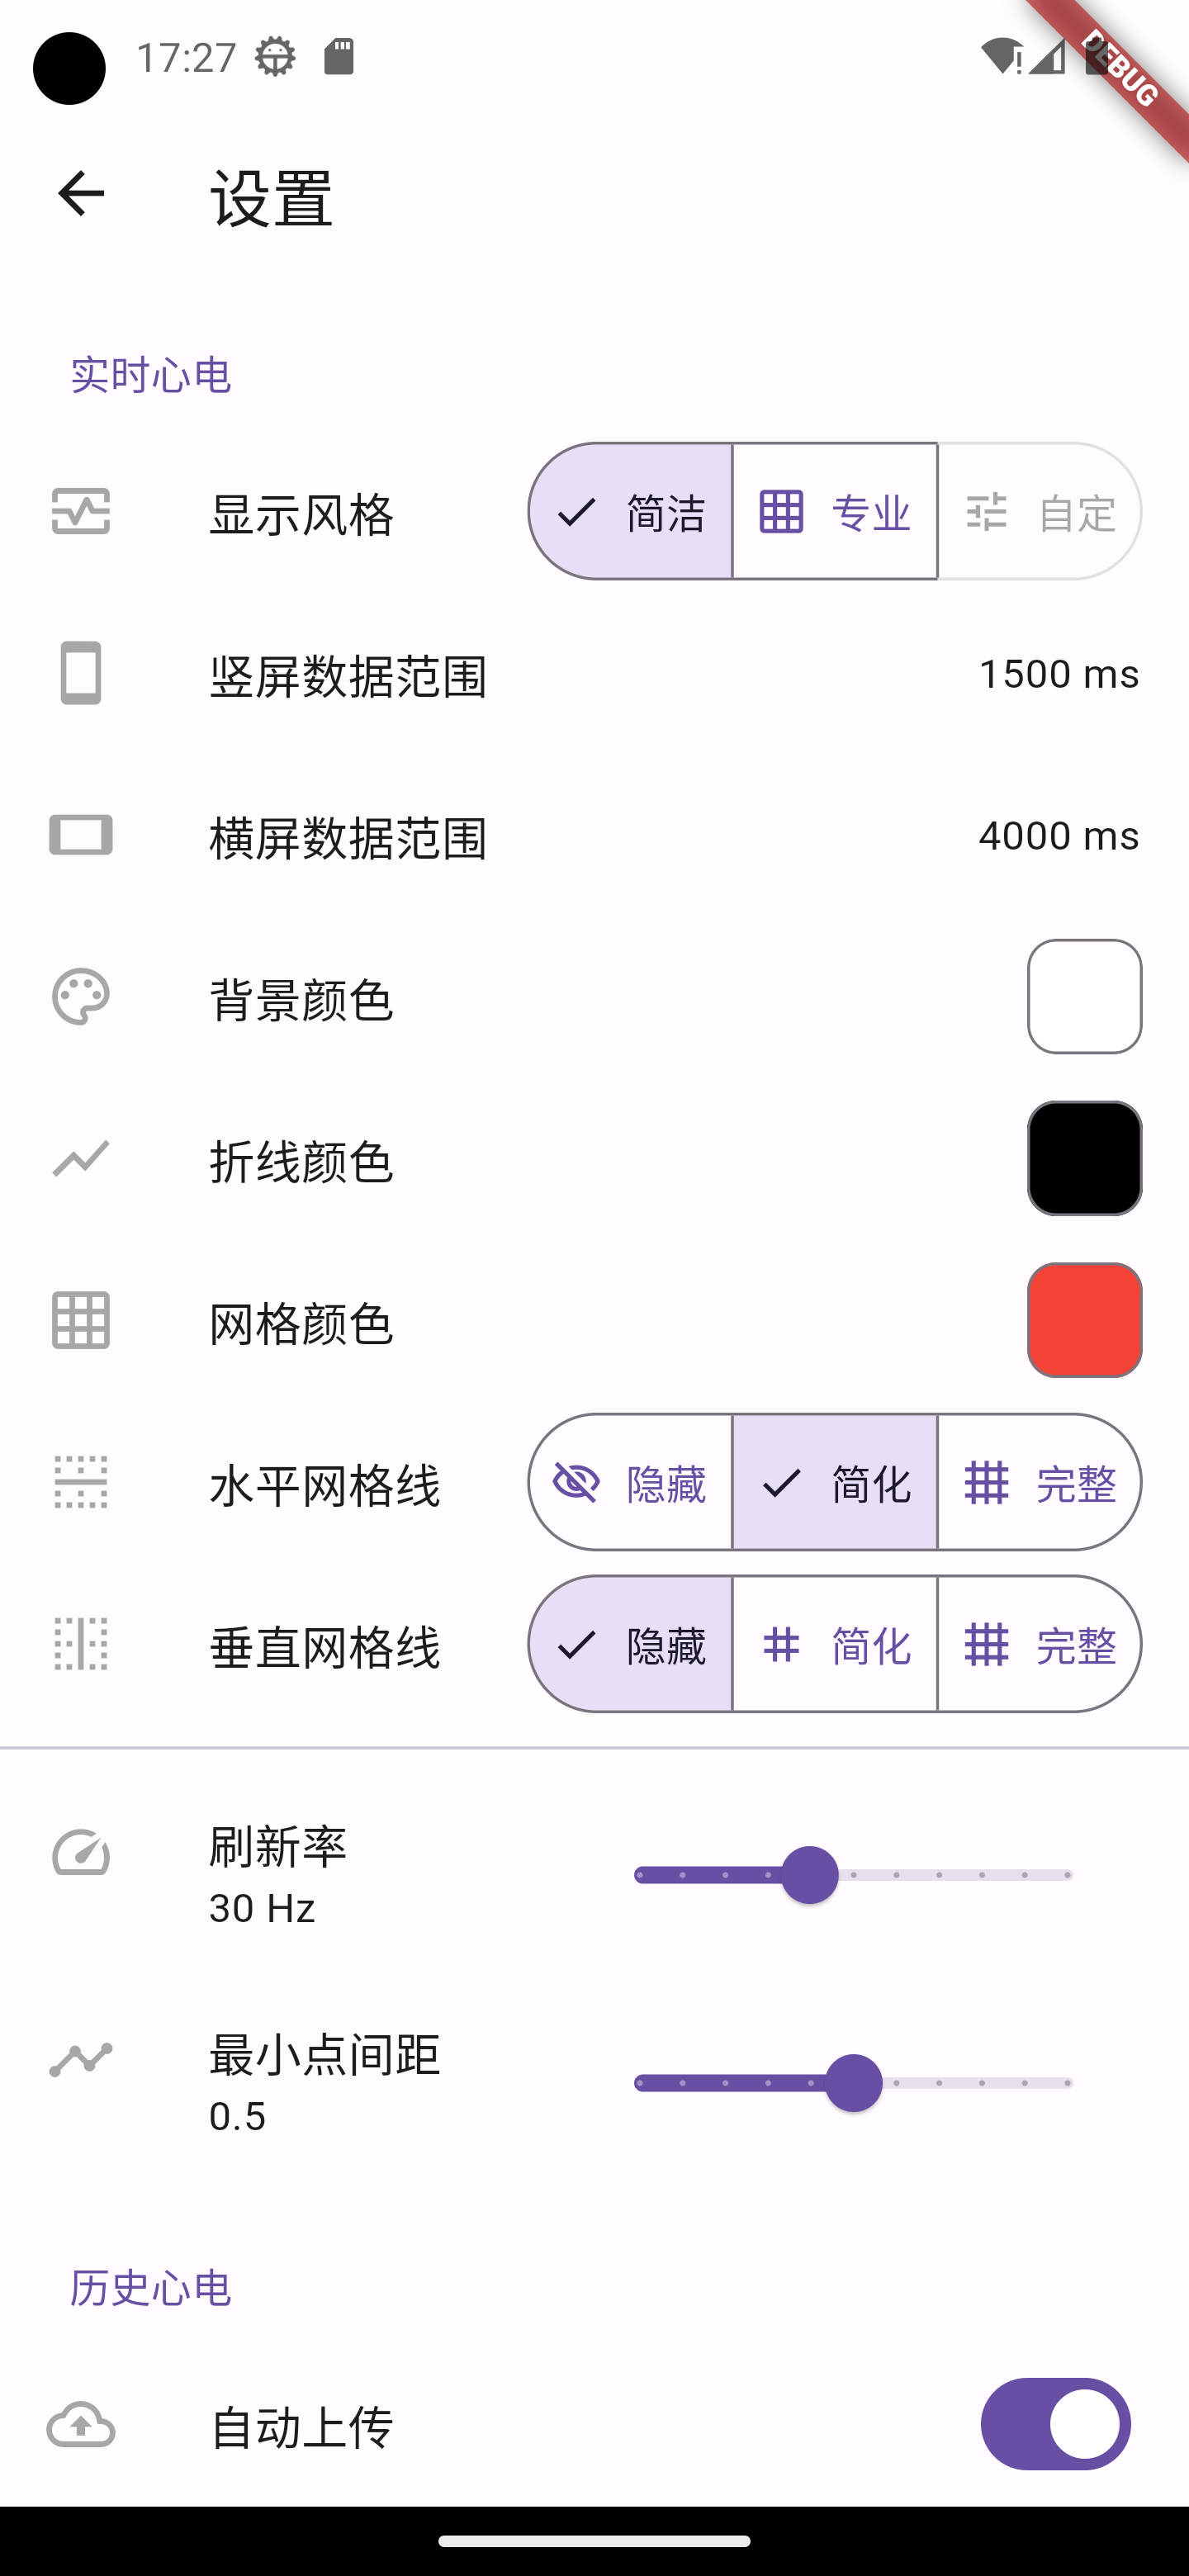
\includegraphics[width=.33\textwidth]{../assets/settings}}
    \subcaptionbox{许可}{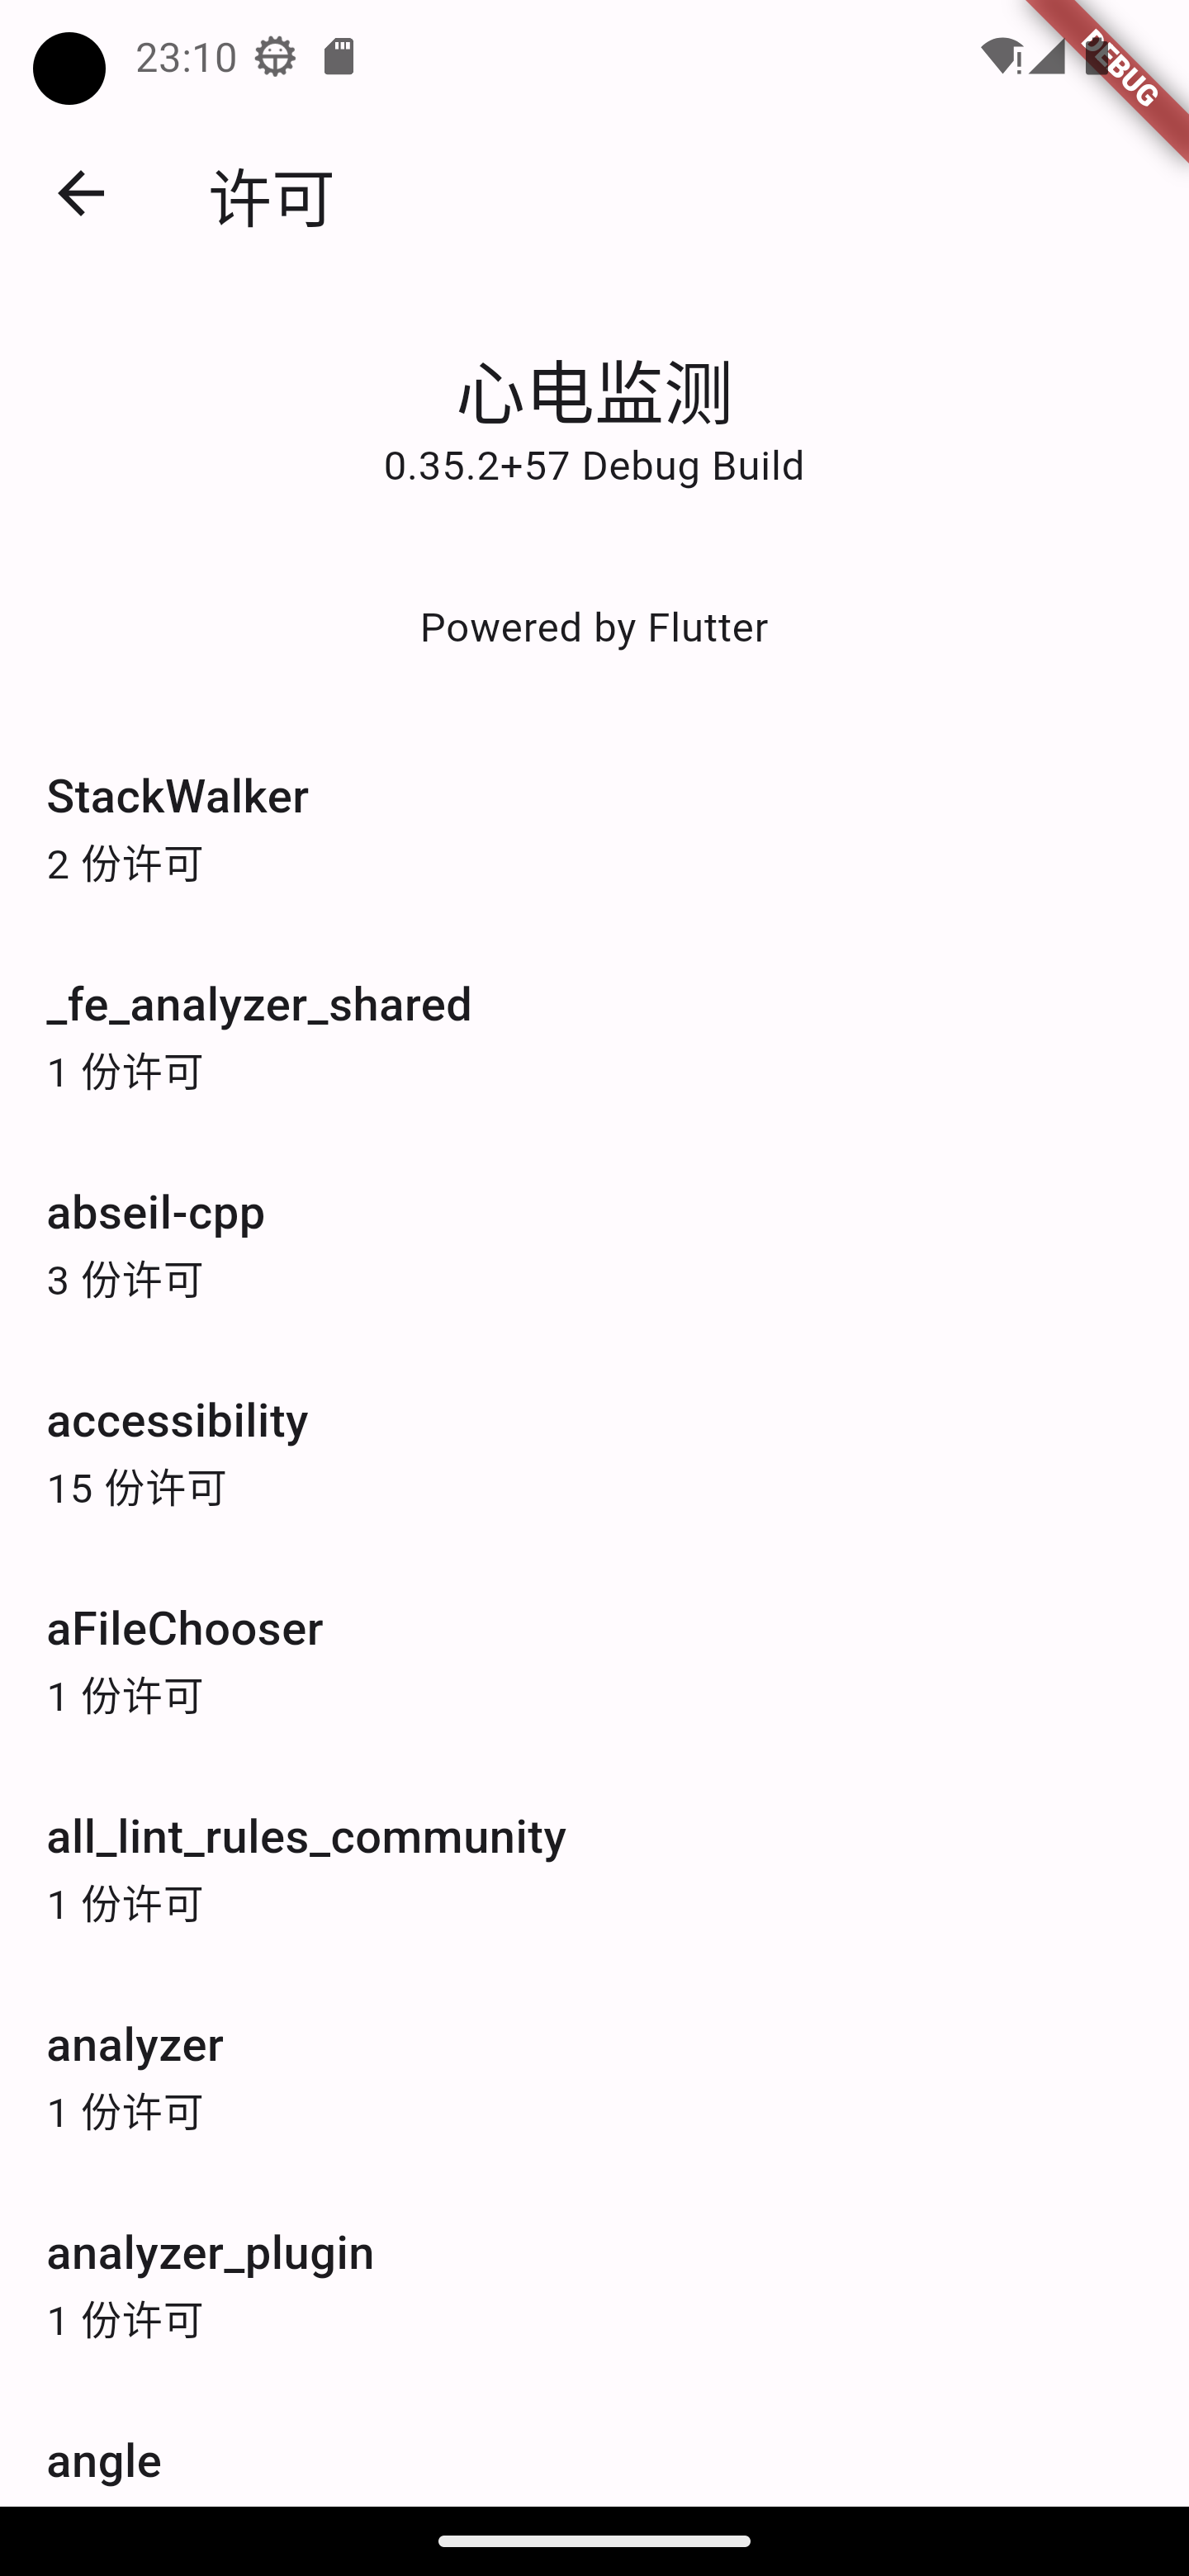
\includegraphics[width=.33\textwidth]{../assets/license}}
    \bicaption{其他界面的截图}{Screenshot of the other pages}
    \label{fig:other}
\end{figure}

\subsubsection{我的界面的设计}\label{subsubsec:me-design}

我的界面提供了其他所有界面的入口,在导航栏中的图标是用户头像的抽象表示。该界面以列表形式展示其内容。用户项目显示了当前用户的头像、姓名、性别、年龄、ID等信息,由于可以复用Web端(同课题下的另一个子项目)的用户管理相关的内容,所以并未对用户界面进行专门设计。反馈、帮助按钮会在点击后打开对应的网页。设置按钮会在点击后打开设置界面。关于按钮会在点击后显示包含应用自身的版本、构建模式等信息的对话框,并提供更新日志与许可信息的入口。

\subsubsection{应用设置界面的设计}\label{subsubsec:settings-design}

应用设置界面为常见的列表形式,划分为多个部分,每部分有一个小标题。设置项目均使用了图标、标题、输入组件的形式来展示,有部分如滑动条等的设置项目因不方便在输入组件直接展示当前状态而添加了副标题。而颜色选择器等所需面积较大的输入组件则有缩小形式与完整形式,缩小形式仅指示当前状态,点击后会在弹出的对话框中显示完整形式。

\subsubsection{许可界面的设计}\label{subsubsec:license-design}

通常而言,用户并不会有查看应用程序所使用的各个开源包的许可协议的需求。但是,由于多数许可协议要求在应用程序中提供许可协议的副本,因此应用程序中必须提供该界面的入口。该界面以列表形式展示其内容。许可界面的每一项都是一个开源包,点击后会在弹出的界面中显示该开源包的名称、作者、许可协议等信息。此外,该界面的上方也显示了本应用的名称、版本和构建模式的信息,并显示了“Powered by Flutter”的标识。

\subsubsection{界面过渡动画的设计}\label{subsubsec:transition-design}

界面过渡动画是连接单个元素或应用程序全屏视图的短动画,是出色的用户体验的基础,可以帮助用户感知到应用程序的界面设计逻辑。由于在无法插入动态图片或视频的情况下较难充分展示界面过渡动画的实际效果,因此本文只作简短说明。

应用在心律类型详情界面的开启与关闭过程中使用了容器转换。当用户点击心律类型区域后,该区域会逐渐扩展至全屏,并将内容渐变为心律类型详情内容,关闭时则反之。这使得各个界面之间的关系清晰明确,加强了分析报告界面与心律类型详情界面的关联感。

在历史心电的所选时间改变后,使用了水平滑动效果,以提醒用户心电图是发生了水平移动。由于各个心拍之间的图像可能较为相似,如果没有该动画,用户可能会产生心电图发生了微小变形而非水平移动了一个心拍的错觉。

点击导航栏跳转至对应界面时使用了顶级(Top level)转换效果。该效果专门用于在应用程序的顶级目的地之间导航时,比如点击导航栏中的按钮时。该效果会将旧屏幕快速淡出,然后新屏幕快速淡入。由于顶级目的地的内容不一定相关,因此该动画效果有意不使用分组或持久元素来在屏幕之间创建牢固的关系。

\subsubsection{数据自动上传与自动删除的设计}\label{subsubsec:data-auto-design}

应用每天会自动上传历史心电数据与分析报告结果至服务器(服务器端属于同课题的另一个子项目)。由于历史心电数据量较大而分析报告数据量较小,应用在设置中为两者的上传提供了分别的开关,以便流量有限的用户可以选择仅上传分析报告。

因为移动设备存储空间较为有限,所以应用会自动删除较旧的数据。应用删除数据的范围是距离当前时间超过两天的数据,而非一天,这是出于两点考虑:其一是因为应用内各界面最远提供了一天前的数据查询功能,如果在查询过程中进行删除,需要进行额外的加锁等考虑,而且可能会导致查询结果不准确;其二是因为应用在自动上传数据时可能会因为网络等原因失败,将数据额外保留一天可以提供一些重试的机会。

\subsubsection{应用的无障碍设计}\label{subsubsec:accessibility-design}

图~\ref{fig:accessibility} 展示了应用的一些无障碍设计。

\begin{figure}[ht]
    \subcaptionbox{界面放大}{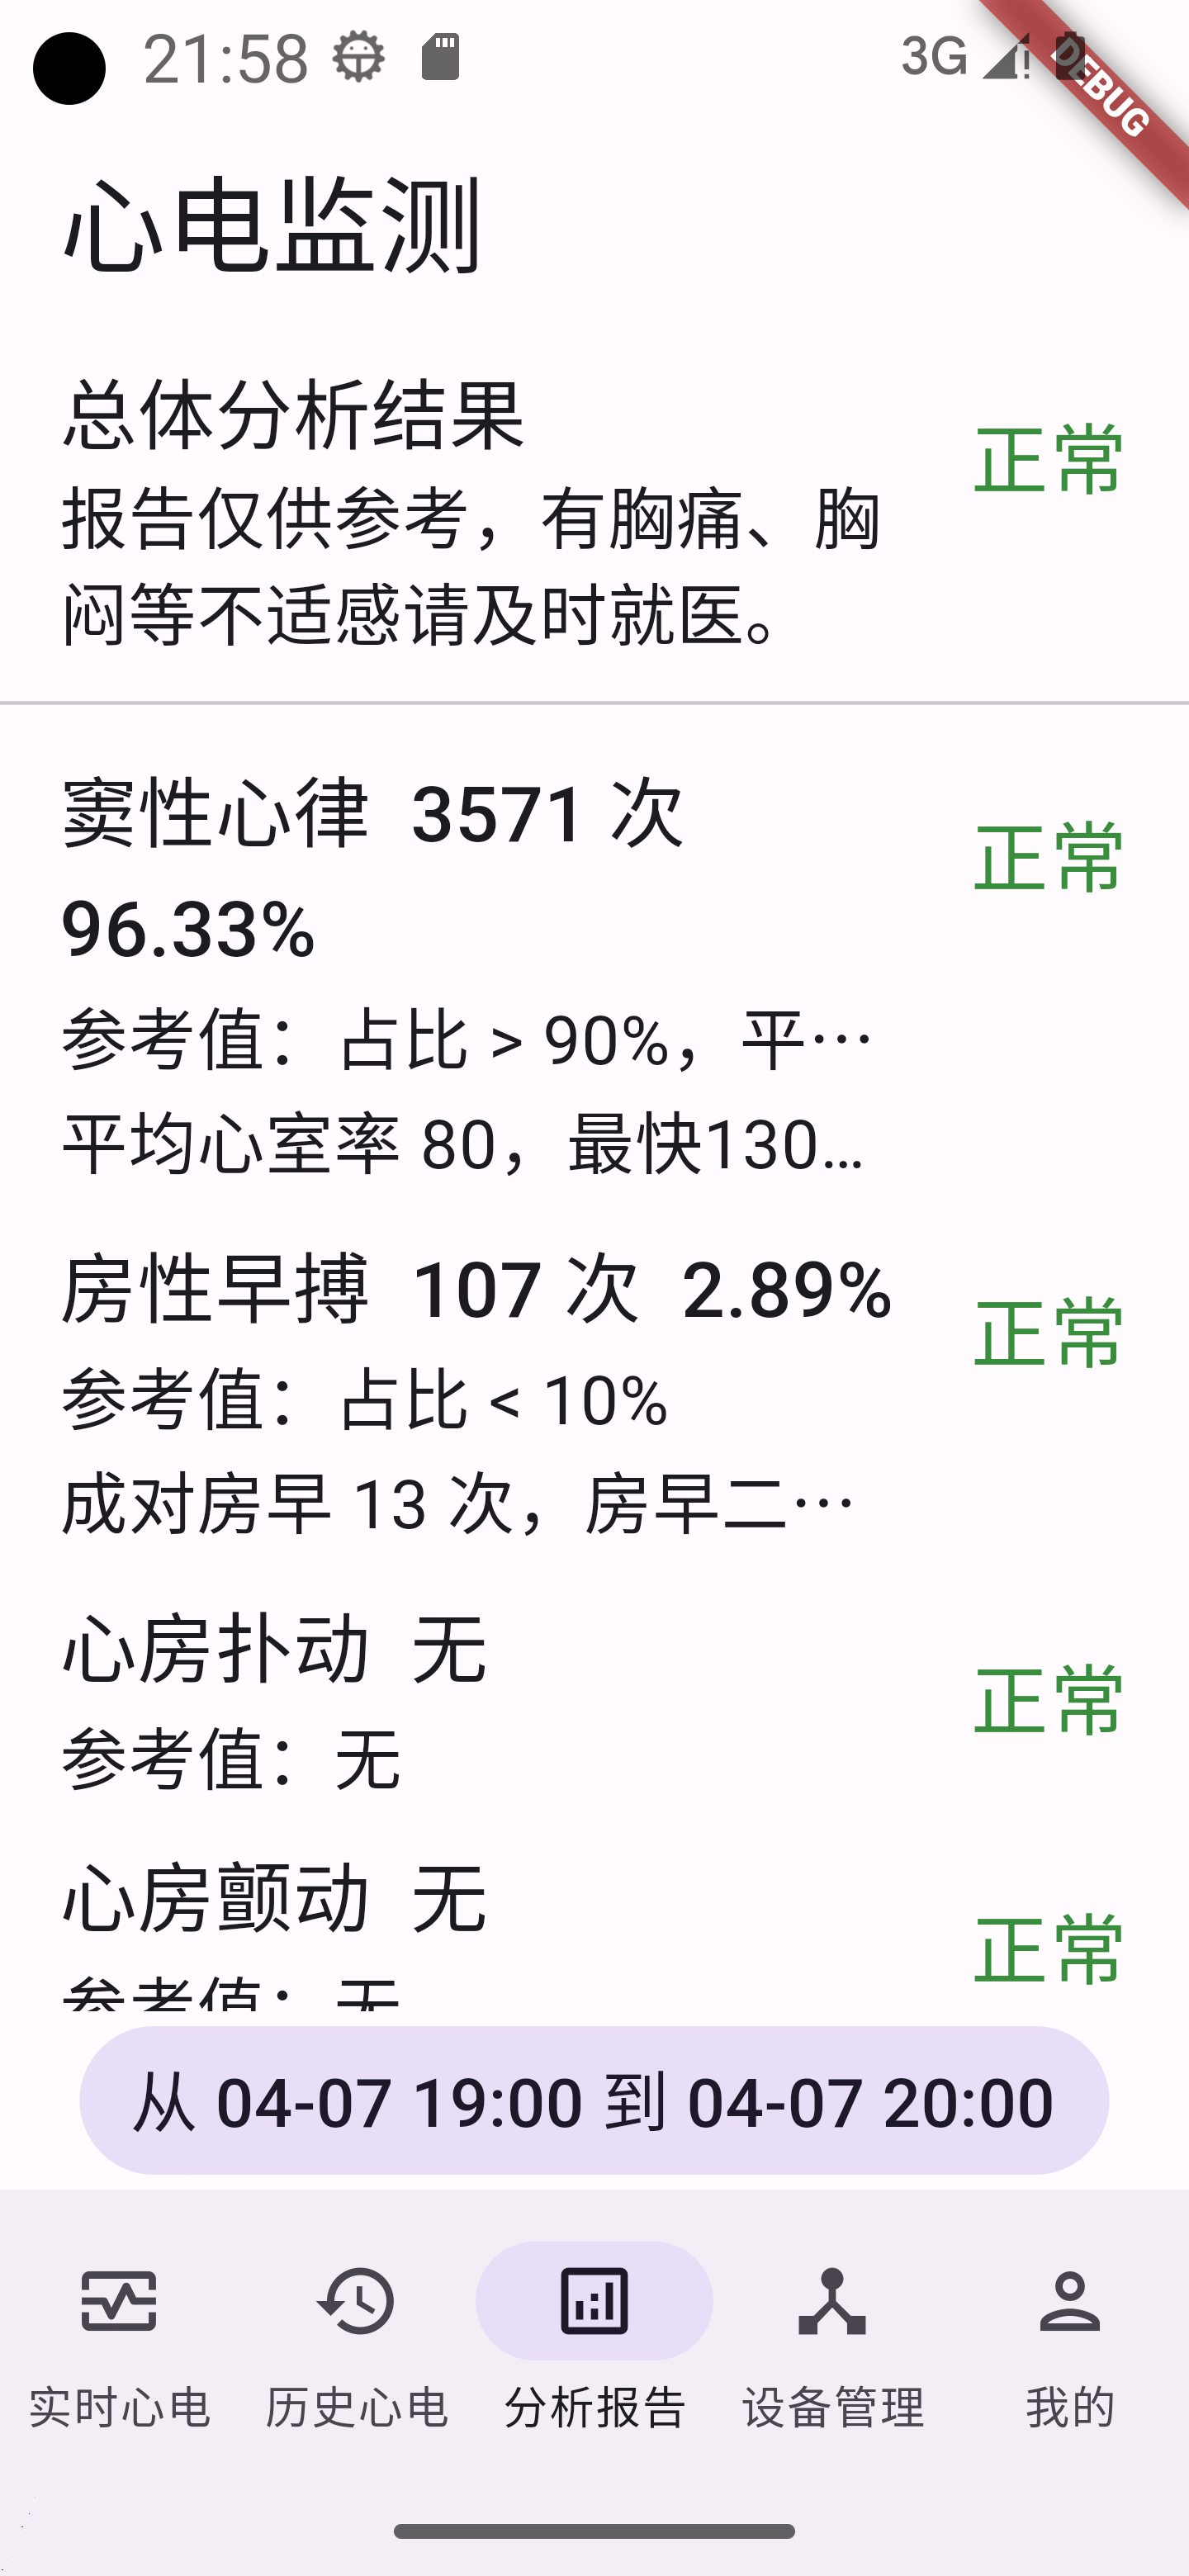
\includegraphics[width=.33\textwidth]{../assets/big}}
    \subcaptionbox{粗体高对比度}{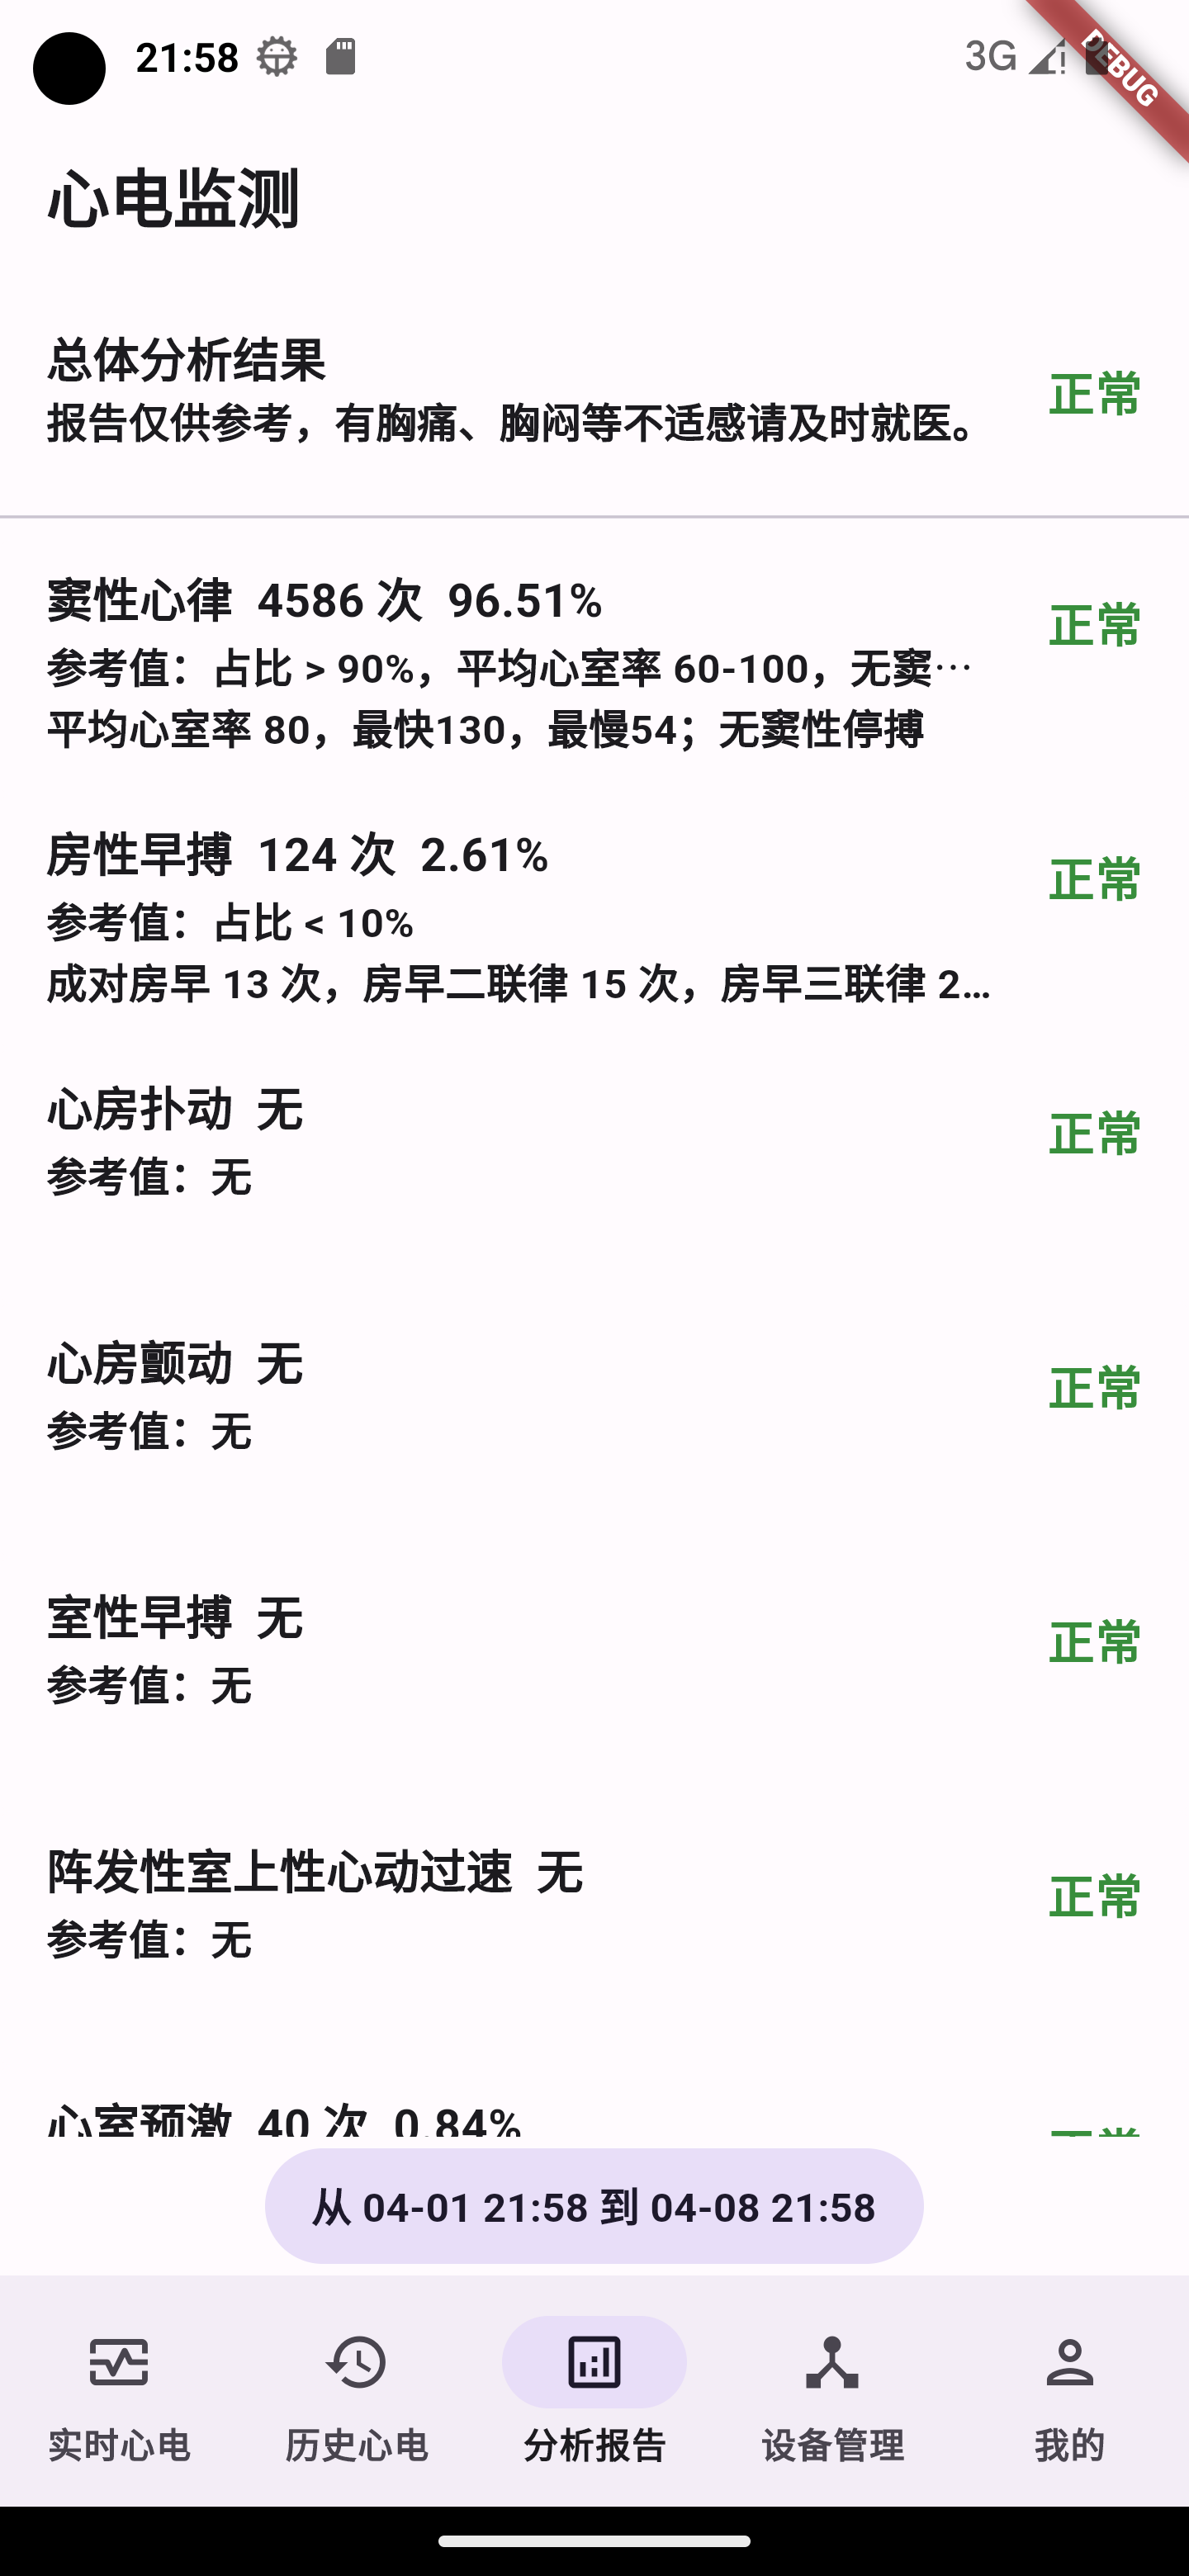
\includegraphics[width=.33\textwidth]{../assets/bold}}
    \subcaptionbox{深色模式}{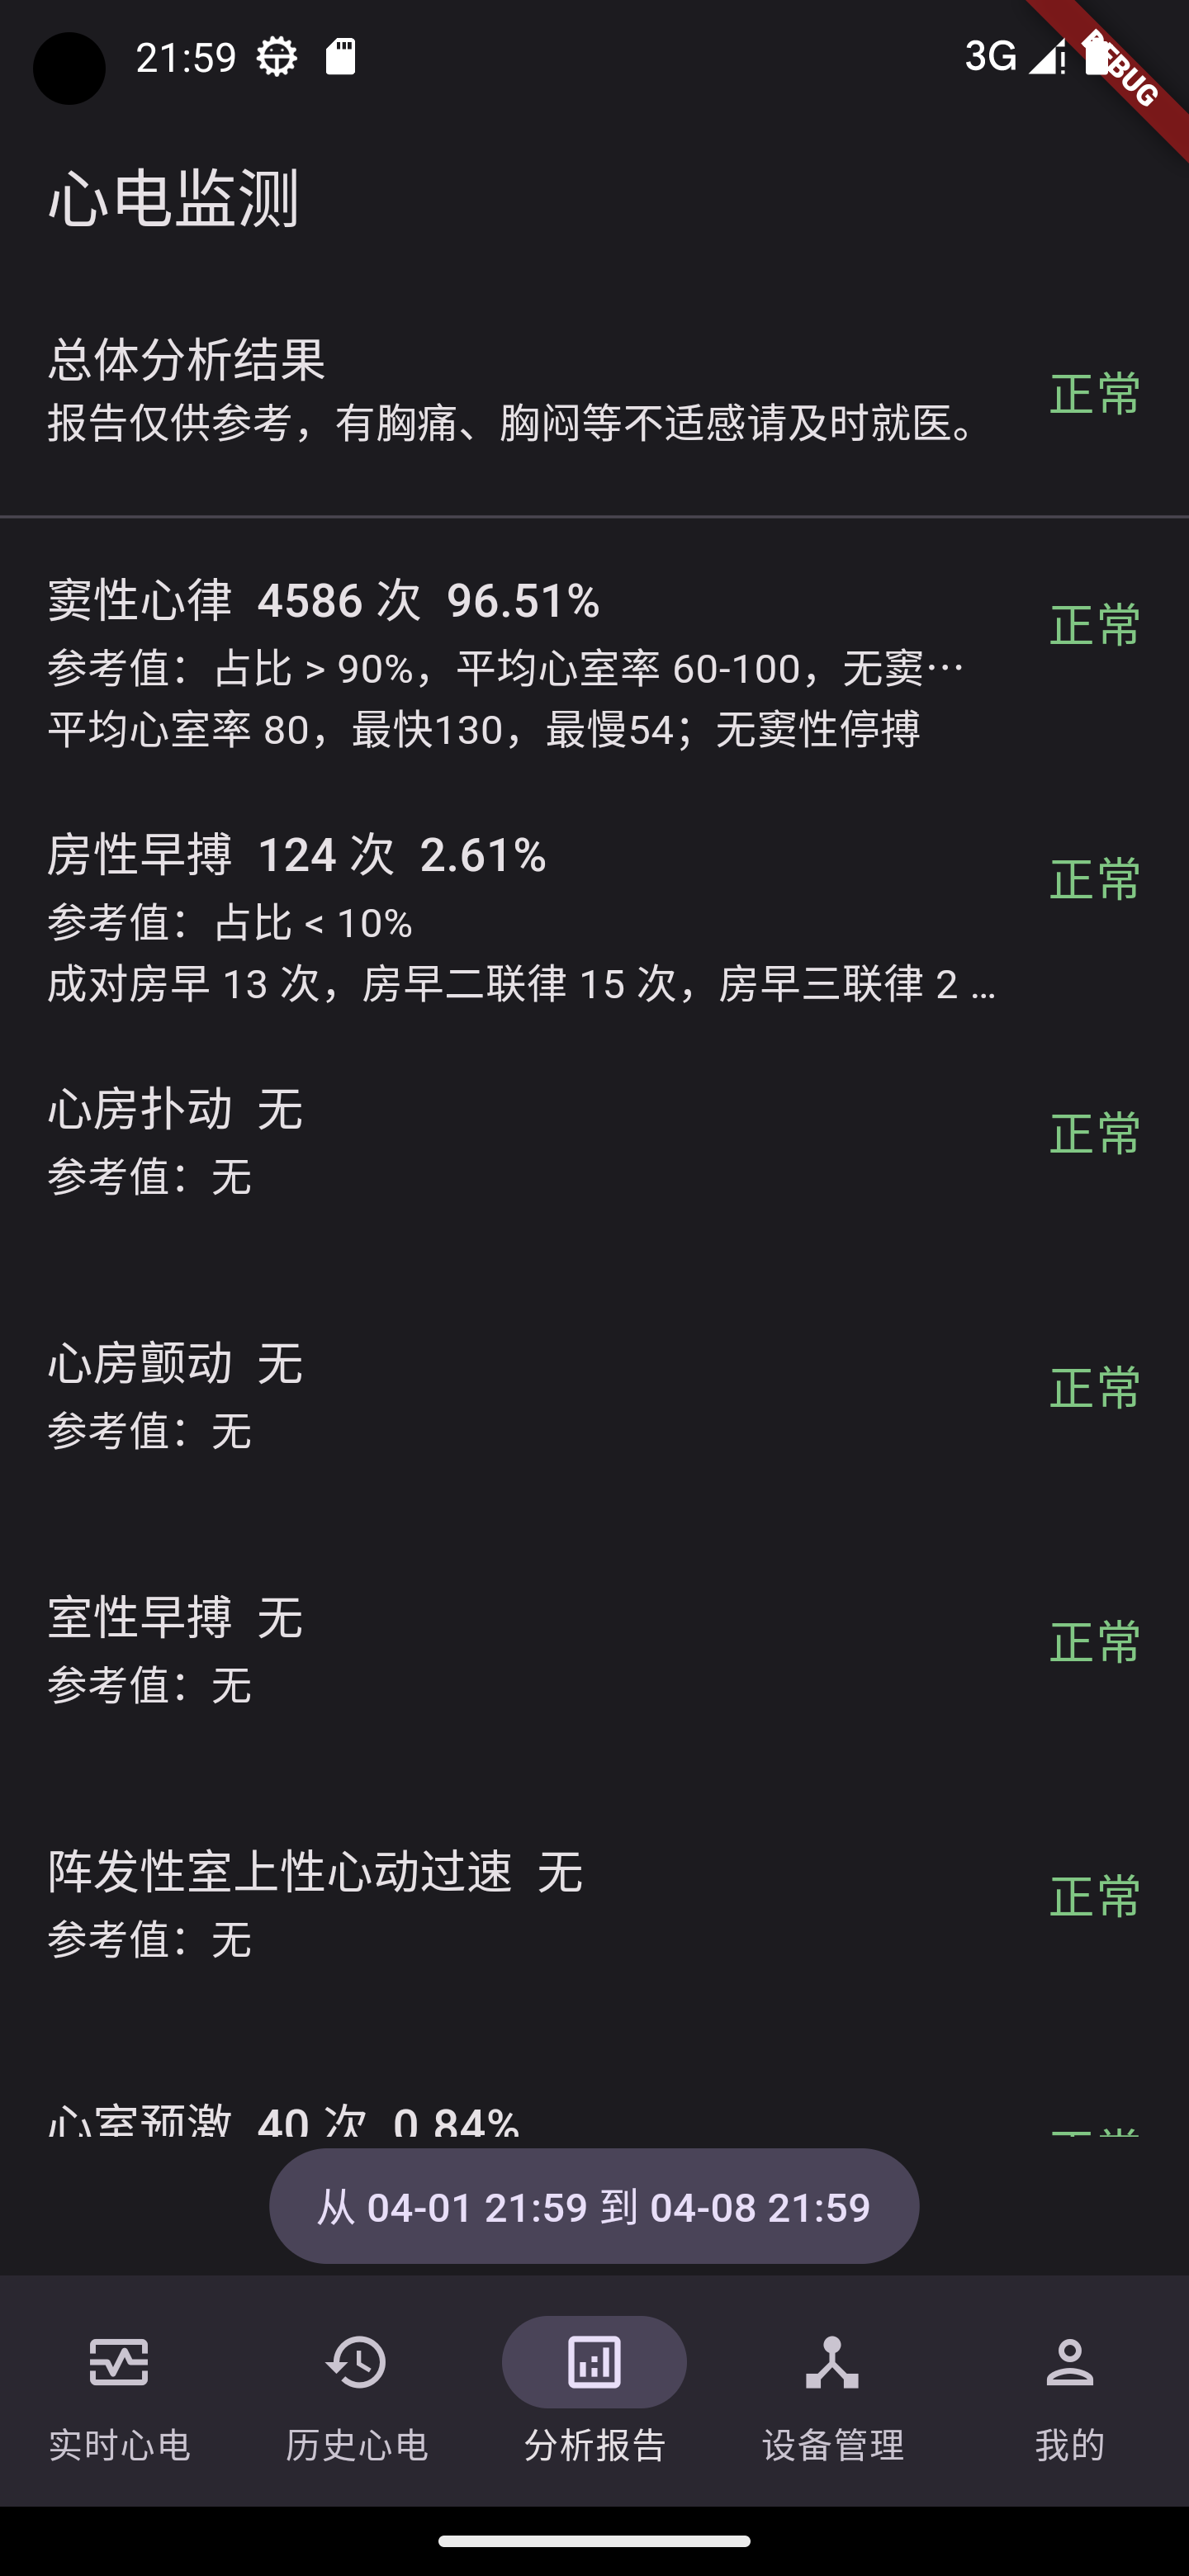
\includegraphics[width=.33\textwidth]{../assets/dark}}
    \bicaption{应用的无障碍设计}{Accessibility design of the app}
    \label{fig:accessibility}
\end{figure}

当用户开启了界面放大后,应用内一些原本在一行之内显示的文本会无法在一行内完整显示。对于有必要完全显示出来的内容,应用会将其进行换行,在多行之中显示。对于没有必要完全显示的内容,应用会将其折叠,以省略号指示内容未显示完全。通过这些设计,应用在界面放大的状态下虽然美观程度略有下降,但功能都可以保证正常使用。界面放大的一个常用替代方式是将文本加粗加黑,应用在这种情况下也可以正常提供功能。

为了支持深色模式与浅色模式的切换,应用在设计中尽量避免了使用固定的颜色,而是使用系统上下文提供的颜色。这样,应用在不同的主题下自然都可以随之自动切换颜色,从而正常显示内容。


\section{应用的数据库设计}\label{sec:db-design}

应用的数据库分为两部分,存储简单数据的SharedPreferences数据库和存储复杂数据的Isar数据库。前者主要用于存储应用的设置,后者主要用于存储历史心电数据与分析报告结果。

\subsection{SharedPreferences数据库的设计}\label{subsec:shared-preferences}

\subsubsection{SharedPreferences数据库介绍}\label{subsubsec:shared-preferences-intro}

SharedPreferences是Flutter的一个包,提供了简单键值对的存储功能,可以视为一个键值型的非关系型数据库。其在Android平台上基于同名的SharedPreferences功能,在iOS上则基于NSUserDefaults功能。

SharedPreferences仅支持少数几种数据类型,即 |int|、|double|、|bool|、|String| 以及 |List<String>|。键值型数据库的读写非常简单,不需要进行特别的设计。本项目对该数据库的设计主要在于将各种需要存储的类型映射为其支持的类型。

\subsubsection{Duration类型的存储}\label{subsubsec:duration-storage}

Duration类型表示时间长度。由于应用内对时间的各种操作最多只需要毫秒精度,所以应用在需要将Duration类型的数据存入SharedPreferences时会将其转换为毫秒数以整数格式进行存储。在读取时,应用会将毫秒数转换为Duration类型。

\subsubsection{Color类型的存储}\label{subsubsec:color-storage}

Color类型表示颜色。应用在需要将Color类型的数据存入SharedPreferences时,会将其编码为32位整数以整数格式进行存储。在读取时,应用会将32位整数转换为Color类型。具体的编码方式是将颜色的ARGB值分别存储在32位整数的高8位、次高8位、次低8位和低8位中。

\subsubsection{枚举类型的存储}\label{subsubsec:enum-storage}

应用中使用了各种枚举类型,有时会需要将枚举类型存入SharedPreferences。应用在存储枚举类型时会将其转换为索引值,以整数形式存储。枚举类型常见的存储方式还包括按其名称以字符串形式存储、为每个枚举值赋予自定义值然后按自定义值的类型存储。相比其他方法,直接按索引值存储的优点在于其简单高效;缺点在于已经存在的枚举值不能轻易改动,否则会破坏已有的数据。由于应用内的枚举值设计基本不变,所以该缺点并不明显,可以接受。

\subsection{Isar数据库的设计}\label{subsec:isar}

\subsubsection{Isar数据库介绍}\label{subsubsec:isar-intro}

Isar是Flutter的一个包,提供了一个跨平台数据库。Isar属于非关系型数据库,不过提供了组合索引、ACID语义、事务等功能,可以视为一个关系型数据库的子集。相比常规的关系型数据库,Isar有一些额外的限制(或者说缺少一些功能)影响了本应用对数据库的设计。

当使用Isar来存储数据时,需要对Collection进行操作。Collection可理解为Isar数据库中的表,其包含的数据只能为同一类Dart对象,每个对象则代表了对应数据表中的一行数据。该类对象所对应的类则是这张表的Schema,其中每个字段对应数据库中的一列。与一般的关系型数据库相同的是,Schema中必须要有主键;不同的是,Isar中主键的类型被限制为64位整数值,这一限制导致了本应用对数据库的设计中的一些不同之处。

在查询时,Isar并不像一般的关系型数据库那样在编写SQL语句后自动生成最优查询策略,而是需要手动指定查询方式。Isar中的查询过滤方式分为两种,分别称为Filter和Where,前者执行遍历过滤,后者依靠索引表进行过滤。多个Where子句的过滤结果直接只能进行并集运算,无法进行交集运算。如果需要按多个属性进行过滤,并且还希望使用索引加快速度,就必须使用组合索引。组合索引有一个特殊的限制:主键不能包含在组合索引之中。这一限制也影响了本应用对数据库的设计。

此外,Isar对外键、Join等功能的支持也比较有限,不过这些功能在本应用的数据库设计中本来也不需要,所以不进行过多说明。

\subsubsection{心拍数据的存储}\label{subsubsec:beat-storage}

在分析报告数据中,只有心拍数据被存入数据库,基于心拍数据产生的进一步分析结果则只在查询时动态生成。这一方面是因为算法的大部分时间开销在于分割分类模型的运行上,其余部分开销较小。另一方面是因为心拍之外的结果的格式较为复杂,不方便进行合适的数据库设计。心拍数据则格式简单,且存储、查询时可以对多段数据进行拼接、裁剪而不失去太多准确度,所以适合存入数据库之中。

心拍数据的Schema包含3个字段和2个索引。字段中的ID是由Isar管理的自增整数,没有特别用途。另外两个字段分别是DateTime类型的心拍时间和枚举类型的心拍类型标签。对心拍时间进行了单列索引,以方便在查看历史心电时快速检索指定时间范围内的所有心拍。对心拍类型和心拍时间进行了组合索引,以心拍类型为主索引,这个组合索引用于查询指定标签在指定时间范围内的数量等信息。

\subsubsection{心电数据的存储}\label{subsubsec:point-storage}

对心电数据的查询需求较为简单,只有在历史心电界面中需要对指定时间范围内的心电数据进行查询。因此,也只需要在心电数据的时间上进行索引。

由于没有组合索引的需求,所以可以直接把时间作为主键,以节省额外的索引表的开销,并避免浪费主键所占的空间。由于主键只能为64位整数,所以需要对时间进行编码。考虑到时间只需要毫秒精度,将其编码为了自Unix纪元(UTC时间的1970年1月1日00:00:00)以来经过的毫秒数。这样,心电数据的Schema中不包含任何额外定义的索引,查询时只使用主键自带的索引功能。

除了作为主键的时间之外,一条心电数据中还包含各导联的电压数据。由于导联I、II、III被定义为左臂、右臂、左腿三个点之间的电位差,这三个导联的数据实际上只包含两个差值的信息量,所以只需要存储两个值即可。
